%% This is file `elsarticle-template-1-num.tex',
%%
%% Copyright 2009 Elsevier Ltd
%%
%% This file is part of the 'Elsarticle Bundle'.
%% ---------------------------------------------
%%
%% It may be distributed under the conditions of the LaTeX Project Public
%% License, either version 1.2 of this license or (at your option) any
%% later version.  The latest version of this license is in
%%    http://www.latex-project.org/lppl.txt
%% and version 1.2 or later is part of all distributions of LaTeX
%% version 1999/12/01 or later.
%%
%% Template article for Elsevier's document class `elsarticle'
%% with numbered style bibliographic references
%%
%% $Id: elsarticle-template-1-num.tex 149 2009-10-08 05:01:15Z rishi $
%% $URL: http://lenova.river-valley.com/svn/elsbst/trunk/elsarticle-template-1-num.tex $
%%
\documentclass[preprint,12pt]{elsarticle}

%% Use the option review to obtain double line spacing
%% \documentclass[preprint,review,12pt]{elsarticle}

%% Use the options 1p,twocolumn; 3p; 3p,twocolumn; 5p; or 5p,twocolumn
%% for a journal layout:
%% \documentclass[final,1p,times]{elsarticle}
%% \documentclass[final,1p,times,twocolumn]{elsarticle}
%% \documentclass[final,3p,times]{elsarticle}
%% \documentclass[final,3p,times,twocolumn]{elsarticle}
%% \documentclass[final,5p,times]{elsarticle}
%% \documentclass[final,5p,times,twocolumn]{elsarticle}

%% The graphicx package provides the includegraphics command.
\usepackage{graphicx}
%% The amssymb package provides various useful mathematical symbols
\usepackage{amssymb}
\usepackage{amsmath}
\usepackage{amsthm}
\usepackage{mathtools} 
\usepackage[utf8]{inputenc}
\usepackage[english]{babel}
\usepackage{multirow}% http://ctan.org/pkg/multirow
\usepackage{graphicx}% http://ctan.org/pkg/graphicx
\usepackage{arydshln}
\usepackage{subcaption} 

%% The lineno packages adds line numbers. Start line numbering with
%% \begin{linenumbers}, end it with \end{linenumbers}. Or switch it on
%% for the whole article with \linenumbers after \end{frontmatter}.
\usepackage{lineno}
\usepackage{stackengine}
\usepackage{scalerel}
\usepackage{fp}
\usepackage{mathtools}
\usepackage{tikz}

\newcommand\tikzmark[1]{%
  \tikz[remember picture,overlay]\coordinate (#1);}
%% natbib.sty is loaded by default. However, natbib options can be
%% provided with \biboptions{...} command. Following options are
%% valid:

%%   round  -  round parentheses are used (default)
%%   square -  square brackets are used   [option]
%%   curly  -  curly braces are used      {option}
%%   angle  -  angle brackets are used    <option>
%%   semicolon  -  multiple citations separated by semi-colon
%%   colon  - same as semicolon, an earlier confusion
%%   comma  -  separated by comma
%%   numbers-  selects numerical citations
%%   super  -  numerical citations as superscripts
%%   sort   -  sorts multiple citations according to order in ref. list
%%   sort&compress   -  like sort, but also compresses numerical citations
%%   compress - compresses without sorting
%%
%% \biboptions{comma,round}

% \biboptions{}

\makeatletter
\newcommand\longleftrightarrowfill@{%
  \arrowfill@\leftarrow\relbar\rightarrow}
\makeatother

\newcommand{\supp}{\mathop{\mathrm{supp}}}
\newcommand{\Bezier}{{B\'{e}zier} }
\newtheorem{lemma}{Lemma}

\journal{Journal Name}

\begin{document}
\graphicspath{{./img/}} 

\begin{frontmatter}

%% Title, authors and addresses

\title{Isogeometric analysis of $C^1/G^1$ dual mortaring and its application for multi-patch Kirchhoff-Love shell}

%% use the tnoteref command within \title for footnotes;
%% use the tnotetext command for the associated footnote;
%% use the fnref command within \author or \address for footnotes;
%% use the fntext command for the associated footnote;
%% use the corref command within \author for corresponding author footnotes;
%% use the cortext command for the associated footnote;
%% use the ead command for the email address,
%% and the form \ead[url] for the home page:
%%
%% \title{Title\tnoteref{label1}}
%% \tnotetext[label1]{}
%% \author{Name\corref{cor1}\fnref{label2}}
%% \ead{email address}
%% \ead[url]{home page}
%% \fntext[label2]{}
%% \cortext[cor1]{}
%% \address{Address\fnref{label3}}
%% \fntext[label3]{}


%% use optional labels to link authors explicitly to addresses:
%% \author[label1,label2]{<author name>}
%% \address[label1]{<address>}
%% \address[label2]{<address>}

\author{Di Miao\\[1cm]{\small Advisor: Michael J. Borden}}
\address{Department of Civil and Environmental Engineering\\
Brigham Young University\\
368 CB, Provo, UT 84602, USA\\}

% \begin{abstract}
% %% Text of abstract
% Suspendisse potenti. Suspendisse quis sem elit, et mattis nisl. Phasellus consequat erat eu velit rhoncus non pharetra neque auctor. Phasellus eu lacus quam. Ut ipsum dolor, euismod aliquam congue sed, lobortis et orci. Mauris eget velit id arcu ultricies auctor in eget dolor. Pellentesque suscipit adipiscing sem, imperdiet laoreet dolor elementum ut. Mauris condimentum est sed velit lacinia placerat. Vestibulum ante ipsum primis in faucibus orci luctus et ultrices posuere cubilia Curae; Nullam diam metus, pharetra vitae euismod sed, placerat ultrices eros. Aliquam tincidunt dapibus venenatis. In interdum tellus nec justo accumsan aliquam. Nulla sit amet massa augue.
% \end{abstract}

% \begin{keyword}
% Science \sep Publication \sep Complicated
% %% keywords here, in the form: keyword \sep keyword

% %% MSC codes here, in the form: \MSC code \sep code
% %% or \MSC[2008] code \sep code (2000 is the default)

% \end{keyword}

\end{frontmatter}

%%
%% Start line numbering here if you want
%%
\linenumbers

%% main text
\section{Introduction}
Isogeometric analysis was introduced by Hughes et. al.~\cite{HUGHES20054135} in 2005, as a novel discretization technology. Since then, it attracted considerable attentions from the acedamic world and is enjoying explosive growth. The idea behind isogeometric analysis is to use the same basis functions for the geometric modeling and computational analysis. While the main aim of isogeometric analysis is to eliminate the geometric approximation error, it has been observed that, compared to traditional $C^0$ finite element, higher regularity Non-uniform Rational B-splines (NURBS) provide higher efficiency per degree of freedom~\cite{bazilevs2006isogeometric, da2011some, da2014mathematical}. Meanwhile, high regularity basis functions allow us to solve higher order partial differential equations (PDEs), e.g. the biharmonic equation~\cite{moore2017discontinuous, kapl_isogeometric_2015, kapl_isogeometric_2017}, the Kirchhoff-Love shell problem~\cite{kiendl2009isogeometric, kiendl2010bending, kiendl2015isogeometric} and the Cahn-Hilliard equation~\cite{gomez2008isogeometric, borden2012phase, borden2014higher}.\par

However, the higher dimensional NURBS basis functions are obtained by a tensor product of one-dimensional NURBS basis functions, which imposes limitations on its feasibility for analysis. Considering a scenario that a refinement is applied to a region of interest, however, for the tensor-product domain, it also introduces control points far from that region, which dramatically increases the problem size. \par

The adaptive finite element technique try to automatically refine a mesh in an optimal fashion so that a desirable discretization error level is achieved with the fewest degrees of freedom. Based on the solution from a coarse mesh, a \textit{posteriori} error estimator provides a guidance for deciding where and how to refine a mesh. It can increase the convergence rate, particularly when singularities are present. However, this promising technique can not be applied directly to NURBS mesh, as it does not support local refinement.\par

Since high smoothness basis function can be used in Isogeometric analysis, the numerical approximation of high order PDEs can be realized in the framework of the standard Galerkin formulation. However, without introducing mesh degenerations, it is impossible to parameterize geometries with sharp corner or kink by high continuity meshes.

\section{Literature review}
To circumvent the shortcomings discussed above, various methods have been proposed. The purpose of this section is to provide an overview of the popular methods that endow B-spline meshes with multi-patch coupling and local refinement abilities. 
\subsection{Local refinable splines}
In 1988, Forsey and Bartels \cite{forsey_hierarchical_1988} introduced the hierarchical B-spline refinement algorithm, which can restrict the influence of refinement to the locality. The algorithm is achieved by a re-representation process that replaces each basis function by an equivalent linear combination of a set of basis functions defined by nested knot vectors. However, due to the lack of a natural control grid, the hierarchical B-spline has not been widely recognized in the CAD society, and a few applications can be found in geometric design. Recently, this technique has been extended to Isogeometric Analysis, by Vuong \textit{et al.} \cite{vuong_hierarchical_2011}. Owing to the construction strategy, the resulted hierarchical basis function are linearly independent and retain the maximal regularity, which renders the hierarchical B-spline a good candidate for analysis. The numerical tests demonstrate that the use of the hierarchical B-spline lead to a superior performance for problems with corner singularity. A subdivision-based hierarchical B-spline was proposed by Bornemann \textit{et al.} \cite{bornemann_subdivision-based_2013}, to tackle the intricate algorithms in the software implementation of hierarchical B-splines. The subdivision scheme establishes algebraic relations between the basis functions and their coefficients defined on different refinement level of the mesh and greatly ease the implementation of hierarchical B-splines. Consecutively, the truncated basis for hierarchical splines (THB-spline) was introduced by Giannelli \textit{et al.} \cite{giannelli_thb-splines:_2012}. THB-splines is created by eliminating from the coarse hierarchical basis function the contribution corresponding to the subset of finer basis functions. Besides all the nice properties of hierarchical B-splines, the THB-splines obtain smaller support and form a partition of unity, which lead to sparser matrices and lower condition numbers. \par

However, all the above hierarchical B-splines are still under the tensor product formulism, which restricts hierarchical B-splines to a global rectangular parametric domain. In order to represent complex topologies, subdivision schemes are widespread in geometry processing and computer graphics. Among the most popular subdivision schems are the Catmull-Clark \cite{catmull_recursively_1978}, Doo-Sabin \cite{doo_behaviour_1978} and Loop's \cite{loop_smooth_1987} scheme. For Isogeometric Analysis, Wei \textit{et al.} \cite{wei_truncated_2015} introduced truncated hierarchical Catmull-Clark subdivion (THCCS) that can handle extraordinary nodes involved in complex topologies. THCCS inherits the surface continuity of Catmull-Clark subdivision, namely $C^1$ continuity at extraordinary points and $C^2$ continuity elsewhere. Loop subdivision surfaces provides similar regularity properties as THCCS and has been applied to Isogeometric Analysis in \cite{kang_truncated_2016,pan_isogeometric_2015} to generate triangular meshes. One of the limitations in the implementation of subdivision meshes is that the basis function around the extraordinary point is composed of piecewise polynomial functions with an infinite number of segments, which leads to insufficient integration by Gauss quadrature rule. To deal with this issue, various quadrature rules and adaptive strategies have been examined in \cite{nguyen_comparative_2014} for Poisson problem on the disk and in \cite{juttler_numerical_2016} for fourth order PDEs. \par

In 2003, Sederberg \textit{et al.} \cite{sederberg_t-splines_2003} introduced T-splines, which allows the existence of T-junctions in the control grid, so that lines of control points need not traverse the entire control grid. Thus, local refinement can be realized by introducing T-junctions around interested region. Since the concept of T-splines is a generalization of NURBS technology, it can be used to merge NURBS surfaces that have different knot-vectors at the intersection. Therefore, the T-splines are also suitable to address trimmed multi-patch geometries. Due to the desirable features of T-splines, Bazilevs \textit{et al.} \cite{bazilevs_isogeometric_2010} explored this technology in Isogeometric Analysis, and numerical results demonstrated its potential for solving structural and fluid problems. By utilizing the B\'ezier extraction operator, a finite element data structure for T-splines \cite{scott_isogeometric_2011} was developed to ease the incorporation of T-splines into existing finite element codes. However, it has been proven \cite{buffa_linear_2010} that the original definition of T-splines is not sufficient to ensure the linear independence of the basis functions. To circumvent this issue, analysis suitable T-splines \cite{li_linear_2012} was developed by applying an additional constraint that no two orthogonal T-junction extensions are allowed to intersect. Subsequently, the mathematical properties of analysis suitable T-splines were studied in \cite{li_analysis-suitable_2013,xin_li_properties_2015}, and it has been sucessfully applied to the boundary element method \cite{scott_isogeometric_2013}. Meanwhile, an adaptive local h-refinement algorithm with T-splines and a local refinement of analysis-suitable T-splines were introduced by D\"{o}fel \textit{et al.} \cite{dorfel_adaptive_2010} and Scott \textit{et al.} \cite{scott_local_2012}, respectively. However, for both algorithm, the refined mesh is not as local as one could hope and this problem might be severe in 3D.\par

\subsection{Multi-patch geometrically continuous functions}

One of the advantages of Isogeometric Analysis is that it provides basis functions with high smoothness, \textit{i.e.} for $p$-th order splines, they enjoy up to $C^{p-1}$ continuity within a single patch. Thus, it is possible to directly discretize differential operators of order higher than 2. However, continuity higher than $C^0$ for multi-patch discretization imposes significant difficulties. The conception of geometric continuity is very important in CAD field \cite{peters_chapter_2002} for designing smooth multi-patch domain containing extraordinary vertices \cite{peters_joining_1992}. In the parametric space, the geometric continuity of order $s$ ($G^s$ continuity) is a weaker continuity constraint as compared to $C^s$ continuity, while it has been proved by Groisser and Peters \cite{groisser_matched_2015} that $G^s$ continuity in the parametric space is equivalent to $C^s$ continuity of the basis function after the parametric mapping. Thus, the construction of $C^s$ isogeometric functions over a $C^0$ parameterization can be interpreted as geometric continuity $G^s$ of the graph parameterization. Bercovier \textit{et al.} \cite{bercovier_smooth_2014} has shown that for multi B\'ezier patches over an unstructured quadrilateral mesh, as long as the order of polynomial is high enough, there always exists the minimal determining set for a $C^1$ continuity construction. Moreover, the resulting basis functions do not contain subdivisions around extraordinary vetices.\par

The case of $G^1$ continuous functions on bilinearly parametrized two-patch B-spline domains was considered by Kapl \textit{et al.} \cite{kapl_isogeometric_2015}, where the $C^1$ basis functions are constructed and analyzed by numerical tests. It is shown that the space dimensionality heavily depends on the parameterization of two bilinear patch, and optimal convergence is observed on biharmonic problem. However, over-constrained $C^1$ isogeometric spaces that causes sub-optimal convergence is also observed for certain configurations (\textit{e.g.} two-patch non-bilinear parameterizations and $C^{p-1}$ continuity within the patches for $p$-th order spline space). A theoretical analysis of the causing of $C^1$ locking is provided in \cite{collin_analysis-suitable_2016}, where the analysis-suitable $G^1$ geometry parameterization, that allows for optimal approximation of $C^1$ isogeometric spaces, is identified and testified by numerical examples. The methods in \cite{kapl_isogeometric_2015} has been extended to bilinearly parameterized multi-patch domains in \cite{kapl_isogeometric_2017}, where the simple explicit formulas for spline coefficients of $C^1$ basis function is derived and nested $C^1$ isogeometric spaces are generated. Recently, Kapl \textit{et al.} \cite{kapl_space_2017,kapl_space_nodate} explored the construction of $C^2$ isogeometric functions on multi-patch geometries and utilized the $C^2$ isogeometric spaces for $6$-th order PDE.\par
Although the geometrically continuous functions circumvent the use of subdivisions for domains with extraordinary vertices, the requirement of $C^0$ parameterization averts local mesh refinement, and lower continuity is required to avoid $C^1$ locking effect. Thus, its implementation can be complex and it may not be a potential candidate for analysis in more general situations.\par

\subsection{Variational approach for domain coupling}
Unlike geometric design, where high continuity basis functions along the intersections of neighboring patches are required for the construction of high quality surface; in analysis, these strong point-wise constraints are unnecessarily rigorous, a good approximation of PDEs can be made even if these constraints are applied in the weak sense. Moreover, the non-conforming multi-patch coupling is allowed, which maintains the flexibility for the choice of meshes when multi-patch discretization is needed. Mathematically, the error estimation of the non-conforming finite element approximation is based on Strang's lemma \cite{brenner_mathematical_2007,strang_analysis_2008}, which says that for the non-conforming discretized PDEs, the distance between exact solution to the discrete one is bounded by the sum of the approximation error and the consistency error. The approximation error measures the failure of discretized finite dimensional space to capture the exact solution, while the consistency error measures the inconsistency between the exact equation and the discretized equation. Various methods have been developed to eliminate the consistency error and recover optimal convergence, among them are the mortar method (Lagrange multiplier method), stablized Lagrange multiplier method, the Nitsche's method and the discontinuous Galerkin (dG) method.\par

To clearly demonstrate these methods, we consider the following Poisson problem with homogenesous Dirichlet boundary conditions
\begin{align}
    \begin{split}
        -\Delta{u}&=f, \qquad \textnormal{in $\Omega$}\\
        u&=0, \qquad \textnormal{on $\partial\Omega$}
    \end{split}\label{eq:poisson_strong}
\end{align}
where $\Omega$ denote a bounded open domain in $\mathbb{R}^d$, $d=2$ or $3$ being the dimension of the problem and its boundary is denoted by $\partial{\Omega}$, in order to simplify the presentation we restrict ourselves to the case of two-dimensional computational domain. The weak form of Equation~\eqref{eq:poisson_strong} reads as follow: Find $u\in{H^1_0(\Omega)}$ such that
\begin{equation}
    a(u,v)=l(v), \qquad \forall v\in{H^1_0(\Omega)},\label{eq:poisson_weak}
\end{equation}
where 
\begin{align}
    \begin{split}
        a(u,v)&=\int_{\Omega}\nabla{u}\cdot\nabla{v}d\Omega,\\
        l(v)&=\int_{\Omega}fvd\Omega.
    \end{split}
\end{align}
Using the fact that $C^0(\Omega)\subset{}H^1(\Omega)$, the weak solution can be approximated by considering a finite dimensional continuous function space. Now, we assume that the domain $\Omega$ is subdivided into $K$ non-overlapping subdomains or patches $\Omega_k$ for $1\leq{k}\leq{K}$, i.e.\ 
\begin{equation}
\bar{\Omega} = \bigcup_{k=1}^{K} \bar{\Omega}_{k}  \quad \textrm{and} \quad {\Omega}_{k}\bigcap{\Omega}_{l}=\emptyset \quad \forall k\neq{l}.
\end{equation}
For simplicity, we only consider the case that the intersection of two patches is either empty or vertex or the entire edge, which rules out the possibility of hanging nodes. We denote the common interface of two neighboring subdomains $\Gamma_{kl}=\partial{\Omega}_k\bigcap\partial{\Omega}_l$ so that $\Gamma_{kl}=\emptyset$ if $\Omega_k$ is not a neighbor of $\Omega_l$ and define the skeleton $\mathbf{S}=\bigcup_{k,l\in{K}, k\neq{l}}\Gamma_{kl}$ as the union of all interfaces. A representative example of geometry is presented in Figure~\ref{fig:patch_partition}. We can associate each subdomain a bijective geometric mapping as
\begin{equation}
  \mathbf{F}_{k}\left(\xi_{k},\eta_{k}\right)\colon{\hat{\Omega}_k}\mapsto{{\Omega}_k}\in\mathbb{R}^d,
\end{equation}
where ${\hat{\Omega}_k}$ is the parametric domain of $k^{th}$ patch associated with coordinates $\left(\xi_{k},\eta_{k}\right)$. For the simplicity and without loss of generality, we assume ${\hat{\Omega}_k}=\left[{0,1}\right]\times\left[{0,1}\right]$ for all patches. Due to the difference in the patch parameterizations, a physical point on the interface can be mapped to different parametric domains with different coordinates. Owing to non-singular parameterization, we can establish a bijective transformation from the shared edge of $\hat{\Omega}_k$ to that of $\hat{\Omega}_l$ by 
\begin{equation}
  \mathbf{E}_{kl}=\left(\mathbf{F}_{l}\right)^{-1}\circ\mathbf{F}_{k}.
\end{equation}
\begin{figure}
    \centering
    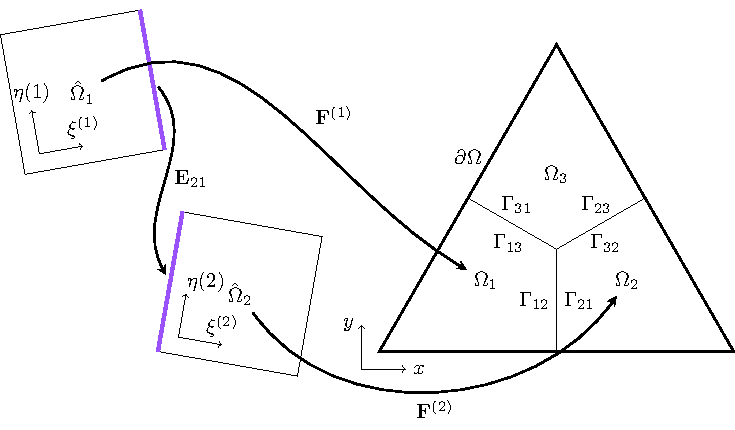
\includegraphics[width=.8\linewidth]{patch_partition}
    \caption{An example of domain decomposition, patches are defined on different parametric domains and are connected via geometric mapping.}\label{fig:patch_partition}
\end{figure}\par
For each $\Omega_k$, we introduce the function space
\begin{equation}
    H^1_*(\Omega_k):=\left\{u\in{}H^1(\Omega_k): u=0\quad\text{on } \partial\Omega\bigcap\partial\Omega_k \right\},
\end{equation}
now we can define the broken Sobolev space 
\begin{equation}
    \mathcal{X}:=\left\{u\in{}L^2(\Omega): u\vert_{\Omega_k}\in{}H^1_*(\Omega_k)\right\}.
\end{equation}\par
Now, the question is how to approximate the weak solution of Equation~\eqref{eq:poisson_weak} from a finite dimensional subspace of $\mathcal{X}$. Since functions in $\mathcal{X}$ can be discontinuous on the skeleton $\mathbf{S}$, $a(u,u)$ is no longer coercive (or V-elliptic) on $\mathcal{X}$. As a result, directly using a finite dimensional subspace of $\mathcal{X}$ to discretize Equation~\eqref{eq:poisson_weak} will lead to a  non-invertible stiffness matrix. Modifications to the weak form is needed, and we will review some of the most popular methods in this section.
\subsubsection{Lagrange multiplier method}
The Lagrange multiplier method (or sometimes called mortar method) is a domain decomposition technique that allows the coupling of different discretization schemes or of non-matching triangulation along interior interfaces. The inter-element continuity condition is enforced weakly by Lagrange multipliers. For the Poisson problem, the $C^0$ continuity constraint is required on the intersections, in other words, the jump on the skeleton
\begin{equation}
    \left[u\right]_{\Gamma_{kl}}:=u_k-u_l=0, \quad \forall \quad\Gamma_{kl}\in\mathbf{S},\label{eq:c0_strong_constrant}
\end{equation}
where $u_k=u\vert_{\Omega_k}$. In order to apply the constraint to the weak form, we introduce the potential energy functional:
\begin{equation}
    \Pi(v):=\frac{1}{2}a(v,v)-l(v).\label{eq:potential_energy}
\end{equation} 
The Equation~\eqref{eq:poisson_weak} is equivalent to the minimization problem:
\begin{equation}
    \inf_{v\in{H^1_0(\Omega)}}\Pi(v).
\end{equation}
Then, given a function space $\mathcal{M}$ defined on the skeleton, a Lagrange multiplier $\mu\in{\mathcal{M}}$ is used to add the constraint~\eqref{eq:c0_strong_constrant} to the potential energy functional~\eqref{eq:potential_energy}, and the resulted the potential energy functional for the Lagrange multiplier method reads
\begin{equation}
    \Pi_{LM}(v,\mu):=\Pi(v)+b(\mu,v),\label{eq:potential_energy_LM}
\end{equation}
where
\begin{equation}
    b(\mu,v)=\sum_{\Gamma\in\mathbf{S}}\int_\Gamma\mu\left[u\right]_{\Gamma}d\Gamma.
\end{equation}
The variational formulation of the Lagrange multiplier problem can be derived from the saddle point problem of the potential energy functional~\eqref{eq:potential_energy_LM}
\begin{equation}
    \inf_{v\in{X}}\sup_{\mu\in{M}}\Pi_{LM}(v,\mu),
\end{equation}
as, find $(u,\lambda)\in{\mathcal{X}}\times{\mathcal{M}}$ such that
\begin{equation}
    \left\{
    \begin{array}{ll}
        a(u,v)+b(v,\lambda)=l(v) \quad \forall v\in{\mathcal{X}},\\
        b(u,\mu)=0 \quad \forall \mu\in{\mathcal{M}}.\label{eq:mixed_form}
    \end{array}
    \right.
\end{equation}
The solution of the variational formulation is the infimum in $v$ and the supremum in $\mu$, in other words, it is still a minimization problem in terms of the primary varible $v$ and any function that violate the constraint will be eliminated by the Lagrange multiplier $\mu$. This is the reason why it is called the saddle point problem. We also denote that the physical meaning of the Lagrange multiplier $\mu$ for~\eqref{eq:potential_energy_LM} is the flux of $v$ over the skeleton. A comprehensive study of the mixed problem~\eqref{eq:mixed_form} can be found in \cite{boffi_mixed_2013}.\par

In the discretized problem, for a given discrete space $\mathcal{X}_h$, the choice of the discrete Lagrange multiplier space $\mathcal{M}_h$ plays a fundamental role for the stability of the saddle point problem and the optimality of the discretization scheme. To ensure the optimality, the function space for Lagrange multiplier should be judiciously chosen so that the consistency error should converges at the same rate as that of the approximation error. The feasibility of the discrete space pair $\mathcal{X}_h\times{}\mathcal{M}_h$ can be measured by the inf-sup test. The inf-sup condition is also refered to as the Ladyzhenskaya-Babuska-Brezzi condition (or simply LBB). It is a crucial condition to ensure the solvability, stability and optimality of a mixed problem. For the problem~\eqref{eq:mixed_form}, the inf-sup condition is \cite{boffi_mixed_2013}, for $v\neq{0}$ and $\mu\neq{0}$
\begin{equation}
    \inf_{\mu\in{\mathcal{M}}}\sup_{v\in{\mathcal{X}}}\dfrac{\vert{b\left({v,\mu}\right)}\vert}{\|{v}\|_{\mathcal{X}}\|{\mu}\|_{\mathcal{M}}}\geq\beta>0.
\end{equation}
Since the approximation error of problem~\eqref{eq:mixed_form} is given as
\begin{equation}
    \|u-u^h\|_{\mathcal{X}}+\|\lambda-\lambda^h\|_{\mathcal{M}}\leq{}C\left({\inf_{u^h\in\mathcal{X}^h}\|u-u^h\|_{\mathcal{X}}+\inf_{\lambda^h\in\mathcal{M}^h}\|\lambda-\lambda^h\|_{\mathcal{M}}}\right),
\end{equation}
where $C$ is a constant that depends on variables including $\beta$ but is independent of the mesh size $h$. Hence, in a discretized problem, the inf-sup condition requires the variable $\beta$ to be a constant that is independent of the mesh size. \par 
It is well-known that in order to satisfy the LBB-condition a number of possible natural choices for the approximation space pair $\mathcal{X}_h\times{}\mathcal{M}_h$ must be discarded. In particular, the trace space of slave side, specially convenient from the computational point of view, often do not satisfy the LBB-condition and can activate pathologies such as spurious oscillations. To remedy this problem, the most widely used method in the finite element framework is reducing the dimension of Lagrange multiplier space by two (for $2^{nd}$ order PDEs). Specifically, the degree of Lagrange multiplier basis functions at both ends are reduced by one. This modification has been sucessfully adopted in \cite{bernardi_basics_2005, bernardi_domain_1993, belgacem_mortar_1998, belhachmi_resolution_1994, belgacem_mortar_1999, marcinkowski1999mortar, lamichhanehigher, belgacem1999extension}. An example of the modified Lagrange multiplier basis functions are illustrated in Figure~\ref{fig:mortar_basis}, where the basis function $N_5$ is constant in the right end.\par

In the context of Isogeometric Analysis, the patch coupling problem has been firstly studied by Hesch and Betsch \cite{hesch_isogeometric_2012}, where the coupling of Lagrangian elements and NURBS elements for 3D nonlinear elastic problem is validated. To avoid an over constrained linear system, Hesch and Betsch used a linear Lagrange multiplier space for higher order NURBS coupling. In \cite{brivadis_isogeometric_2015}, the choice of the Lagrange multiplier space has been extensively studied, it testifies that for equal order pairing, a local degree reduction at extraordinary vertices is required, and another possibility is reducing the degree of Lagrange multiplier space  by two compared to the trace space of slave side. These choices of Lagrange multiplier spaces are proven to be inf-sup stable by various numerical examples. In addition to the constraint on the inter-patch displacement, Bouclier \textit{et al.} \cite{bouclier_development_2017} considered the constraint on the traction and claimed that this strategy enables to present a $C^1$ behavior. In the numerical test, smoother displacement fields and smoother stress fields are observed. \par
\begin{figure}
    \centering
    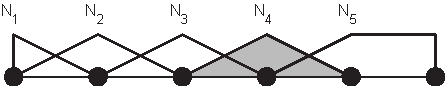
\includegraphics[width=.7\linewidth]{mortar_basis}
    \caption{Lagrange multiplier basis functions for the piecewise linear elements, modification on the right end (from Zienkiewicz \cite{zienkiewicz1977finite}).}\label{fig:mortar_basis}
\end{figure}
Another drawback of the implementation of mortar methods is that most of them introduce Lagrange multipliers as additional variables to enforce interface constraints weakly, increasing the problem size. Moreover, different physical fields are involved in the weak form, deteriorating the conditioning of the global matrix if no appropriate pre-conditioner is applied (detailed discussion about preconditioning for saddle point problem can be found in \cite{farhat_scalable_1995,benzi_preconditioning_2008,tezaur_analysis_1998}).\par

\subsubsection{Dual mortar method}
To circumvent the increase of problem size, we considering the minimization problem 
\begin{equation}
    \inf_{v\in{\mathcal{K}}}\Pi(v), \label{eq:dual_mortar}
\end{equation}
where the function space $\mathcal{K}=\left\{{v\in{\mathcal{X}}\colon{b(v,\lambda)=0, \forall\lambda\in{\mathcal{M}}}}\right\}$. The minimization problem~\eqref{eq:dual_mortar} is indeed equivalent to the saddle point problem~\eqref{eq:mixed_form}, the proof can be found in \cite{boffi_mixed_2013}. Note that, since $K\subset{X}$, the introduce of Lagrange multiplier indeedly reduces the problem size of~\eqref{eq:dual_mortar}. Meanwhile, the symmetric positive definite structure of the resulting stiffness matrix is preserved. But the construction of the function space $K$ is not a trivial task.\par
To reduce the cost of constructing the function space $\mathcal{K}$, we use the dual basis functions of the trace space of the slave side as the discrete Lagrange multiplier space. For a given basis function $N_i$, the dual basis function $\hat{N}_j$ is defined to satisfy
\begin{equation}
    \int_\Gamma{N_i\hat{N}_j}d\Gamma=\delta_{ij}\int_\Gamma{}N_id\Gamma,
\end{equation}
where $\delta_{ij}$ is a Kronecker delta function. Of special interest, are biorthogonal basis functions with compact support, especially
\begin{equation}
    \supp{\hat{N}_i}=\supp{{N}_i}.
\end{equation}
Due to the biorthogonality, the discrete bilinear form $b(v,\mu)$ forms a diagonal matrix on the slave side, and forms a sparse matrix on the master side. The function space $\mathcal{K}$ can be formulated without additional efforts and all the slave degree of freedom are eliminated in the resulting linear system. Moreover, owing to the local support property the resulting stiffness matrix is a symmetric positive definite sparse matrix. Thus, the dual basis functions are very attractive in the perspective of computational efficiency. 

Figure \ref{fig:dual_mortar_basis} shows an example of dual basis functions corresponding to the basis functions in Figure \ref{fig:mortar_basis}. Again, order reduction is made at the right end. The dual mortar method was first introduced in \cite{wohlmuth_mortar_2000} for first order finite element. This method has been extended to higher order degree elements in \cite{lamichhane2002higher}, to three-dimensional problem in \cite{wohlmuth2002comparison} and to contact problem \cite{hueber2005primal, popp2009finite}.\par

\begin{figure}
    \centering
    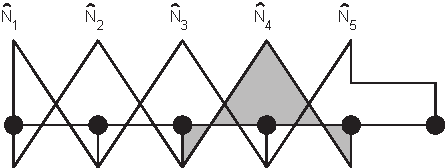
\includegraphics[width=.7\linewidth]{dual_mortar_basis}
    \caption{Dual Lagrange multiplier basis functions for the piecewise linear elements, modification on the right end (from Zienkiewicz \cite{zienkiewicz1977finite}).}\label{fig:dual_mortar_basis}
\end{figure}

In isogeometric analysis framework, a master-slave type mortar method has been suggested by Dornisch \textit{et al.} \cite{dornisch_weak_2015}, where the weakly applied constraint is represented as a master-slave relation and the the slave interface degrees of freedom (DOF) can be condensed out of the global linear system. Recently, Dornisch \textit{et al.} extended this research to multiple patch coupling in \cite{dornisch_patch_2016,dornisch_dual_2017}, where different types of dual basis functions are applied as the basis of Lagrange multipliers. The numerical results demonstrate that the approximate dual basis functions yield accurate result and generate sparse global matrix due to the local support. The concept of dual mortar methods is also utilized in \cite{seitz_isogeometric_2016} for contact problem in Isogeometric analysis framework. Coox \textit{et al.} \cite{coox_robust_2017} proposed an interesting approach to establish the master-slave mortar method and implemented this approach in \cite{coox_isogeometric_2017} to form boundary element analysis on complex manifold. In this approach, the master-slave relation are formed by knot insertion algorithm and pseudo-inverse. \par

\subsubsection{Perturbed Lagrangian method}
Applying constraint by Lagrange multiplier leads to a saddle point problem, of which the discrete Lagrange multiplier basis functions cannot be chosen independently of that of primal variable and special treatment is required on the cross point to ensure the solvability and optimality of the discretized system. The stiffness matrix for the discrete problem arising from the Lagrangian multiplier method always contains both positive and negative eigenvalues, for which iterative methods are known to be less efficient than for symmetric positive definite systems. To ensure the invertibility of the stiffness matrix, a quadratic penalty term is added to the energy functional~\eqref{eq:potential_energy_LM}, as

\begin{equation}
    \Pi_{PLM}(v,\mu):=\Pi_{LM}(v,\mu)-\frac{1}{2\epsilon}\sum_{\Gamma\in\mathbf{S}}\int_\Gamma\mu^2d\Gamma,\label{eq:potential_energy_PLM}
\end{equation}
where the penalty term is scaled by a parameter $\epsilon$. The resulted functional~\eqref{eq:potential_energy_PLM} is refered to as perturbed Lagrangian and the last term is often called stablization term. The resulted variational formulation is stated as
\begin{equation}
    \left\{
    \begin{array}{ll}
        a(u,v)+b(v,\lambda)=l(v) \quad \forall v\in{\mathcal{X}},\\
        b(u,\mu) - \frac{1}{2\epsilon}\sum_{\Gamma\in\mathbf{S}}\int_\Gamma\mu\lambda{}d\Gamma=0 \quad \forall \mu\in{\mathcal{M}}.\label{eq:perturbed_mixed_form}
    \end{array}
    \right.
\end{equation}
As $\epsilon\rightarrow\infty$, the solution obtained from~\eqref{eq:perturbed_mixed_form} will converge to the solution obtained by the classical Lagrange multiplier method. For $0<\epsilon<{\infty}$, any solution that inconsistent with the constraint will not be fully prohibited, but will be penalized by the stability term. And the rank of discrete stiffness matrix is preserved no matter whether the discrete space pair $\mathcal{X}_h\times{}\mathcal{M}_h$ fulfills the inf-sup condition or not. However, for a moderate $\epsilon$, the perturbed Lagrangian method is inconsistent with the classical Lagrange multiplier method, and the increase of $\epsilon$ will deteriorate the conditioning of stiffness matrix.\par

The perturbed Lagrangian method has been utilized in \cite{simo1985perturbed} for contact problem and \cite{dornisch2011boundary, apostolatos2015domain} for domain decomposition problem in isogeometric analysis framework.
\subsubsection{Stablized Lagrange multiplier method}
To fully circumvent the inf-sup condition for imposing Dirichlet boundary by Lagrange multiplier, Barbosa et. al. \cite{barbosa1991finite} added a new penalty like term to the energy functional~\eqref{eq:potential_energy_LM} to enhance the stability. Unlike perturbed Lagrangian method where the penalty term is inconsistent with the original problem, the new term proposed by Barbosa maintaining the consistency. The energy functional of stablized Lagrange multiplier method is given as
\begin{equation}
    \Pi_{SLM}(v,\mu):=\Pi_{LM}(v,\mu)-\sum_{\Gamma\in\mathbf{S}}\frac{h}{2\gamma}\int_\Gamma(\mu+\left\{\frac{\partial{v}}{\partial{n}}\right\})^2d\Gamma,\label{eq:potential_energy_SLM}
\end{equation}
where $n$ is the normal vector of the interface, $h$ is the mesh size on the intersection, $\gamma$ is a user defined constant, the average operator
\begin{equation}
    \left\{u\right\}_{\Gamma_{kl}}:=\frac{1}{2}u_k+\frac{1}{2}u_l.
\end{equation}
Since the physical meaning of the Lagrange multiplier is the flux on the intersection, the stabilization term in~\eqref{eq:potential_energy_SLM} is consistent with the original problem. The resulted variational formulation is stated as
\begin{equation}
    \left\{
    \begin{array}{ll}
        a(u,v)+b(v,\lambda)-\frac{h}{\gamma}\sum_{\Gamma\in\mathbf{S}}\int_\Gamma\frac{\partial{v}}{\partial{n}}(\lambda+{\left\{\frac{\partial{u}}{\partial{n}}\right\}})d\Gamma=l(v) \quad \forall v\in{\mathcal{X}},\\
        b(u,\mu) - \frac{h}{\gamma}\sum_{\Gamma\in\mathbf{S}}\int_\Gamma\mu(\lambda+{\left\{\frac{\partial{u}}{\partial{n}}\right\}})d\Gamma=0 \quad \forall \mu\in{\mathcal{M}}.\label{eq:stablized_mixed_form}
    \end{array}
    \right.
\end{equation}
The stabilization parameter $\gamma$ needs to be carefully chosen. If $\gamma$ is too large, the method degrades to a penalty-type method, with sub-optimal accuracy in the asymptotic limit. If $\gamma$ is too small, the method becomes unstable. Recall the trace inequality
\begin{equation}
    \|h^{\frac{1}{2}}\frac{\partial{u}}{\partial{n}}\|_{\partial{\Omega_{k}}}^2\leq{C}\|\nabla{u}\|_{{\Omega_{k}}}^2.\label{eq:trace_inequality}
\end{equation}
It has been shown \cite{juntunen2015connection} that the mixed formulation~\eqref{eq:stablized_mixed_form} fulfills the inf-sup condition if $\gamma>2C$. The constant $C$ can be approximated by discretize the norms in the inequality~\eqref{eq:trace_inequality} and solve the resulting discrete eigenvalue problem. \par

It has been demonstrated that there is a close connection with the stablized Lagrange multiplier method and Nitsche's method in the context of setting the Dirichlet boundary conditions \cite{stenberg1995some} and in the context of domain decomposition \cite{hansbo2005lagrange, hansbo_nitsches_2005, juntunen2015connection}. Tur et. al. \cite{tur2015modified} utilized this method to solve both small and large deformation contact problems and obtained optimal convergence rate for linear elements. To our knowledge, this method has not been applied in the isogeometric analysis framework yet.
\subsubsection{Discontinuous Galerkin method}
Discontinuous Galerkin method (or Nitsche's method) was introduced in 1971 \cite{nitsche_uber_1971} for handling Dirichlet boundary conditions in the weak sense. Discontinuous Galerkin method resembles a mesh-dependent penalty method. Unlike the standard penalty method, which is not consistent unless the penalty coefficient goes to infinity, discontinuous Galerkin method is consistent with the original problem. Moreover, no additional unknown (Lagrange multiplier) is needed and no discrete inf-sup condition must be fulfilled, contrarily to mixed methods. Meanwhile, additional term are added into the weak form to ensure the ellipticity of the problem.\par
To develop the weak form of discontinuous Galerkin method for homogeneous Poisson problem, we start by multiplying~\eqref{eq:poisson_strong} by a test function $v\in{X}$ and integrating by parts, we obtain
\begin{equation}
    a(u,v)-\sum_{\Gamma\in\mathbf{S}}\int_\Gamma\left\{\frac{\partial{u}}{\partial{n}}\right\}\left[v\right]d\Gamma=l(v).\label{eq:origin_discontinuous_galerkin}
\end{equation}
However, if we consider the right-hand side as a bilinear form, it is not coercive. In other words, this problem is not well-posed, since coercive implies the uniqueness of solution. Meanwhile, this bilinear form is not symmetric. To recover the symmetry and coercivity of the bilinear form, additional terms are needed. To maintain the consistency, the added terms must vanish for the true solution. This lead to the following weak form: find $u\in{X}$ such that
\begin{equation}
\begin{split}
    a(u,v)-\sum_{\Gamma\in\mathbf{S}}\int_\Gamma\left\{\frac{\partial{u}}{\partial{n}}\right\}\left[v\right]d\Gamma-\epsilon\sum_{\Gamma\in\mathbf{S}}\int_\Gamma\left\{\frac{\partial{v}}{\partial{n}}\right\}\left[u\right]d\Gamma+\\
    \sum_{\Gamma\in\mathbf{S}}\frac{\gamma}{h}\int_\Gamma\left[u\right]\left[v\right]d\Gamma=l(v)\quad \forall v\in{\mathcal{X}}.
\end{split}
\end{equation}
Since $\left[u\right]=0$ on the intersections, the above formulation is consistent with~\eqref{eq:origin_discontinuous_galerkin}. Furthermore, and as already stated in \cite{riviere2008discontinuous} the parameter $\epsilon$ can be set to some particular values, namely:
\begin{itemize}
    \item For $\epsilon=+1$, the resulting method is called the symmetric interior penalty Galerkin (SIPG) method. The stiffness matrix of SIPG is symmetric.
    \item If $\epsilon=0$, we obtain the incomplete interior penalty Galerkin (IIPG) method. It involves only a few terms and is of easiest implementation.
    \item If $\epsilon=-1$, the resulting method is called the nonsymmetric interior penalty Galerkin (NIPG) method. It admits one unique solution and converges optimally irrespectively of the value of $\gamma>0$.
\end{itemize}
For $\epsilon=0$ and $\epsilon=+1$, the bilinear form is coercive if $\gamma>C$ and $\gamma>2C$, respectively \cite{riviere2008discontinuous}. Similar to the stablized Lagrange multiplier method, the discontinuous Galerkin method also requires to solve an eigenvalue problem to determine the value of $\gamma$.\par

Discontinuous Galerkin method has been widely studied in various aspects, including imposing boundary condition \cite{hansbo_nitsches_2005}, domain decomposition \cite{becker_finite_2003} and contact problem \cite{chouly_symmetric_2015}. In the field of Isogeometric analysis, Discontinuous Galerkin method has been utilized to imposing Dirichlet boundary condition for trimmed spline meshes \cite{embar_imposing_2010}. The first article discussing discontinuous Galerkin method based domain decomposition strategy was written by Apostolatos \textit{et al.} \cite{apostolatos_nitsche-type_2014}. Nguyen \textit{et al.} extended it to three-dimensional problems in \cite{nguyen_nitsches_2014}. Guo \textit{et al.} \cite{guo_nitsches_2015} proposed a Nitsche's method for coupling Kirchhoff-Love NURBS shell patches. Since the governing equation for Kirchhoff-Love shell is $4$-th order PDE, $C^1$ continuity constraint in imposed weakly in the method. \par

Although discontinuous Galerkin method does not introduce additional DOF and does not need the judicious choice of mutiplier function space, the value of the constants in the stablizing term need to be determined. Normally, they are determined by solving a eigenvalue problem on the domain of the combination of all intersections, which leads to extra computational cost. Meanwhile, the additional stablizing terms reduce the sparsity of the global linear system. For higher order PDEs, discontinuous Galerkin method becomes more complex as higher order derivatives exists in the tractions.\par
A comparison of the variational coupling methods discussed above is shown in Table.~\ref{tab:methods_compare}.
\begin{table}
    \caption{Property comparison of Lagrange multiplier, dual mortal, perturbed Lagrange multiplier, stablized Lagrange multiplier and discontinuous Galerkin methods.}
	\centering
    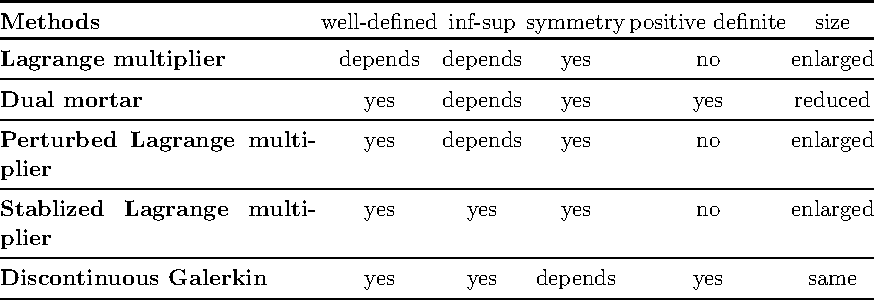
\includegraphics[width=\linewidth]{methods_compare}\label{tab:methods_compare}
\end{table}
\section{Research Objectives}
My dissertation research focuses on the construction of NURBS basis functions among multi-patches that are analysis-suitable for $4^{th}$ order PDEs. The coupling constraints are applied weakly by using the dual mortar method. The dual basis functions are constructed based on the \Bezier probjection technology proposed in \cite{thomas2015bezier}. 
\section{Preliminaries}
This section provides the formulation of univariate basis functions, its extention to higher dimensional space, and representations of geometries in the context of Isogeometric Analysis. For a detailed explanation we refer to.
\subsection{Univariate B-spline basis functions}
A univariate B-spline is peicewise polynomial curve represented as a linear combination of B-spline basis functions. Basis functions of $p^{th}$ order B-spline with $n$ degrees of freedom can be defined by a non-decreasing set of real numbers
\begin{equation}
\Xi = \left\{{\xi_1,\xi_2,\cdots,\xi_{n+p+1}}\right\},
\end{equation}
which is called knot vector. B-splines that are interpolatory at the ends can be achieved by requiring the multiplicity of $p+1$ for the first and the last knot. Associated B-spline basis functions are defined using the Cox-de Boor recursion formula:
\begin{gather}
N_{i,0}(\xi)=\begin{cases}1 & \xi_i\leq{\xi}\leq{\xi_{i+1}}\\0 & otherwise \end{cases} \\
N_{i,p}(\xi)=\dfrac{\xi-\xi_i}{\xi_{i+p}-\xi_i}N_{i,p-1}(\xi)+\dfrac{\xi_{i+p+1}-\xi}{\xi_{i+p+1}-\xi_{i+1}}N_{i+1,p-1}(\xi)
\end{gather}
\subsection{Univariate NURBS basis functions}
The univariate Non-Uniform Rational B-spline (NURBS) can describe objects that cannot be represented by polynomial basis, such as circular arcs. NURBS are built from B-splines by dividing each B-spline basis functions by a weight function
\begin{equation}
W(\xi)=\sum_{j=1}^n w_jN_{j,p}
\end{equation}
and multiplying each B-spline basis functions by the associated weight coefficient for the partition of unity. Thus, the NURBS basis functions are defined as:
\begin{equation}
R_{i,p}(\xi)=\dfrac{w_iN_{i,p}}{W(\xi)}
\end{equation}
\subsection{Multivariate basis functions}
For higher dimensional spaces, the B-spline and NURBS basis functions can be formed by the Kronecker product of vectors of univariate basis functions. For a two-dimensional parametric space, given polynomial orders of $p_\xi$, $p_\eta$ and degrees of freedom $n_\xi$, $n_\eta$ in $\xi$, $\eta$ direction, the bivariate B-spline basis functions are defined as:
\begin{equation}
N_{a,\mathbf{p}}(\xi,\eta)=N_{i,p_\xi}(\xi)N_{j,p_\eta}(\eta),
\end{equation}
where the index $a$ is defined by the map
\begin{equation}
a=n_\eta{i}+j.
\end{equation}\par
The bivariate NURBS basis functions are defined as
\begin{equation}
    R_{a,\mathbf{p}}(\xi,\eta)=\frac{w_{a}N_{a,\mathbf{p}}}{\sum_{i=1}^{n}{w_{i}N_{i,\mathbf{p}}}},
\end{equation}
where $n=n_\xi\times{}n_\eta$. 
With some abuse of notation, we will drop the dependency on the polynomial oder and use $N_{i}$ to denote both NURBS basis functions and B-spline basis functions in the rest of the paper.\par
\section{Weak-$C^1$ coupling for two-patch planar domains}
To ground our approach in a practical example, we consider a biharmonic problem on a two-patch planar domain, as demonstrated in Figure.~\ref{fig:two_planar_patches}. The domain $\Omega$ is decomposed to the slave subdomain $\Omega_s$ (with finer mesh on the interface) and the master subdomain $\Omega_m$ (with coarser mesh on the interface). \par
In order of focusing on the coupling algorithm itself, we assume the boundaries that neighboring to the common intersection to be homogeneous Neumann boundaries (north and south of $\Omega_s$ and east and west of $\Omega_m$) and the rest to be homogeneous Dirichlet boundaries (west of $\Omega_s$ and south of $\Omega_m$), denoted by $\Gamma_N$ and $\Gamma_D$ respectively. Then, the strong form of the two-patch biharmonic boundary value problem writes:
\begin{align}
    \begin{split}
        \Delta^2u=f&,\quad \text{in }\Omega, \\
        u=\frac{\partial{u}}{\partial{\mathbf{n}}}=0&, \quad \text{on }\Gamma_D, \\
        \Delta{u}=\frac{\partial{\Delta{u}}}{\partial{\mathbf{n}}}=0&, \quad \text{on }\Gamma_N.
    \end{split}\label{eq:strong_biharmonic}
\end{align}

\begin{figure}
    \centering
    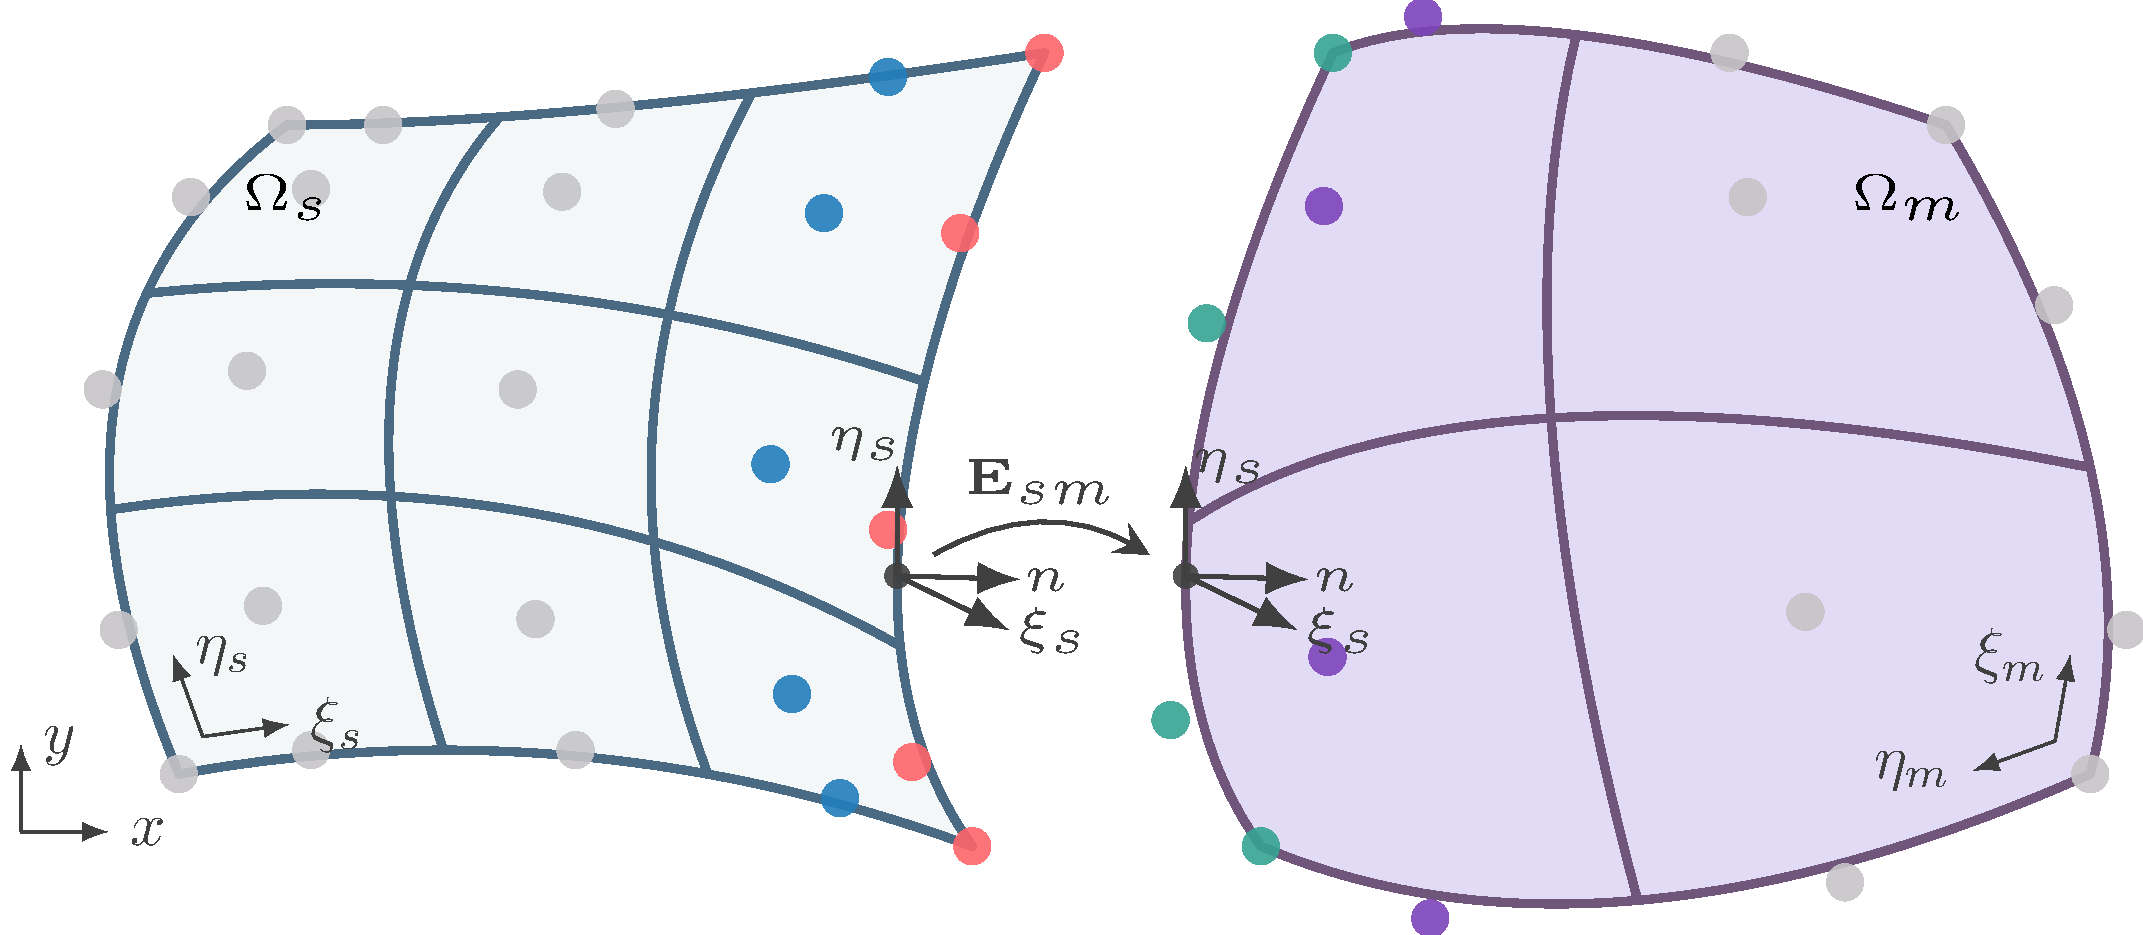
\includegraphics[width=\linewidth]{two_planar_patches}
    \caption{A two-patch planar domain constituted by $\Omega_m$ and $\Omega_s$.}\label{fig:two_planar_patches}
\end{figure}
\subsection{Continuity constraints}
The weak solution of the biharmonic problem~\eqref{eq:strong_biharmonic} is in the space $H^2(\Omega)$. Due to the inclusion $C^1(\Omega)\subset{}H^2(\Omega)$, we can use $C^1$-continuous functions to approximate the solution. For the two multi-patch domain, constraints should be added to compromise the discontinuity along the intersection. In general, the following two constraints are requested for $u$ to be $C^1$-continuous
\begin{subequations}
    \begin{align}
        [u]_{\Gamma_{sm}}&=0,\label{eq:biharmonic_c0}\\
        [\frac{\partial{u}}{\partial{\mathbf{n}}}]_{\Gamma_{sm}}&=0,\quad\text{with }\mathbf{n}=\mathbf{n}_s=-\mathbf{n}_m\label{eq:biharmonic_c1}
    \end{align}
\end{subequations}
where $\mathbf{n}_k$ is the outward normal direction of $\partial{\Omega_k}$.\par
Whereas the constraint~\eqref{eq:biharmonic_c0} can easily fit into the framework of dual mortar method, the constraint~\eqref{eq:biharmonic_c1} can not be directly imposed. First of all, the existence of dual basis functions of $\frac{\partial{N_i}}{\partial{\mathbf{n}}}\vert_{\Gamma_{sm}}$ is doubtful. Even if they exist, as they are biorthogonal to the normal derivative of NURBS, their formulation must depend on the parameterization of $\Gamma_{sm}$, which violates the virtue of simplicity of dual basis functions. Hence, we need the following result, of which the derivatives are defined in the parametric domain and the dual basis functions can be formulated in an elegant manner.\par
\begin{lemma}
    Given two differentiable bijective geometric mappings $\mathbf{F}_{s}\colon\hat{\Omega}_s\rightarrow{\Omega}_s$ and $\mathbf{F}_{m}\colon\hat{\Omega}_m\rightarrow{\Omega}_m$, a $C^0$-continuous function $u$ is $C^1$-continuous in the physical domain if and only if
    \begin{equation}
        [\frac{\partial{u}}{\partial{\mathbf{\xi}_s}}]_{\Gamma_{sm}}=0\text{ and }[\frac{\partial{u}}{\partial{\mathbf{\eta}_s}}]_{\Gamma_{sm}}=0. \label{eq:biharmonic_c1}
    \end{equation} 
\end{lemma}
     
\begin{proof}
    It suffices to consider two neighboring patches as shown in Figure. \ref{fig:two_planar_patches}. $u$ is $C^0$-continuous function implies $[\frac{\partial{u}}{\partial{\mathbf{\eta}_s}}]_{\Gamma_{sm}}=0$. For the $C^1$-continuity of $u$, we have the following relation 
    \begin{align}
        \begin{cases}
            \frac{\partial{u_s}}{\partial{x}}=\frac{\partial{u_m}}{\partial{x}}\\
            \frac{\partial{u_s}}{\partial{y}}=\frac{\partial{u_m}}{\partial{y}}
        \end{cases}
        \xLeftrightarrow{[\frac{\partial{u}}{\partial{\mathbf{\eta}_s}}]_{\Gamma_{sm}}=0}
        \begin{cases}
            \frac{\partial{u}_s}{\partial{\xi_s}}\frac{\partial\xi_s}{\partial{x}}=\frac{\partial{u_m}}{\partial{\xi_s}}\frac{\partial\xi_s}{\partial{x}}\\
            \frac{\partial{u}_s}{\partial{\xi_s}}\frac{\partial\xi_s}{\partial{y}}=\frac{\partial{u_m}}{\partial{\xi_s}}\frac{\partial\xi_s}{\partial{y}}
        \end{cases} \quad \text{on $\Gamma_{sm}$}
    \end{align}
    Since the geometric mapping $\mathbf{F}_s$ is bijective, there exist an inverse mapping $\mathbf{F}_s^{-1}$ and $\det({\mathbf{F}_s^{-1}})\neq{0}$. Thus, $[\frac{\partial{u}}{\partial{\mathbf{\xi}_s}}]_{\Gamma_{sm}}=0$. This concludes the proof.
\end{proof}
The derivatives of $u_m$ w.r.t. $\xi_s$ and $\eta_s$ can be obtained following the chain rule, as
\begin{align}
    \begin{bmatrix}
        \tfrac{\partial{u_m}}{\partial{\xi_s}}\\
        \tfrac{\partial{u_m}}{\partial{\eta_s}}
    \end{bmatrix}
    =
    J(\mathbf{E}_{sm})^T\cdot
    \begin{bmatrix}
        \tfrac{\partial{u_m}}{\partial{\xi_m}}\\
        \tfrac{\partial{u_m}}{\partial{\eta_m}}
    \end{bmatrix},
\end{align}
where $J(\cdot)$ is the Jacobian of the mapping in the argument. The Jacobian of the composition mapping $\mathbf{E}_{sm}$ can be written as
\begin{equation}
    J(\mathbf{E}_{sm})=J(\left(\mathbf{F}_{m}\right)^{-1}\circ\mathbf{F}_{s})=J(\left(\mathbf{F}_{m}\right)^{-1})\cdot{}J(\mathbf{F}_{s})=J(\mathbf{F}_{m})^{-1}\cdot{}J(\mathbf{F}_{s}).
\end{equation}
\subsection{Lagrange multiplier formulation and dual mortar formulation}
We introduce two Lagrange multiplier spaces: $M_0$ is devoted to the $C^0$ constraint~\eqref{eq:biharmonic_c0} and $M_1$ is devoted to the $C^1$ constraint~\eqref{eq:biharmonic_c1}. The Lagrange multiplier formulation of the weak problem of~\eqref{eq:strong_biharmonic} reads: find $u\in{X_b}$, $\lambda_0\in{M_0}$ and $\lambda_1\in{M_1}$ such that:
\begin{align}
    \begin{cases}
        a_b(u,v)+b_0(\lambda_0,v)+b_1(\lambda_1,v)=l(v),\quad\forall v\in{X_b};\\
        b_0(\mu_0,u)=0, \quad\forall \mu_0\in{M_0};\\
        b_1(\mu_1,u)=0, \quad\forall \mu_1\in{M_1};
    \end{cases}\label{eq:biharmonic_mixed}
\end{align}
with
\begin{align}
    a_b(u,v)&=\int_\Omega\Delta{u}\Delta{v}d\Omega,\\
    b_0(\mu,u)&=\int_{\Gamma_{sm}}\mu\left[u\right]_{\Gamma}d\Gamma,\\
    b_1(\mu,u)&=\int_{\Gamma_{sm}}\mu\left[\frac{u}{\xi_s}\right]_{\Gamma}d\Gamma.
\end{align}
The broken Sobolev space for the biharmonic problem is given as
\begin{equation}
    \mathcal{X}_b:=\left\{u\in{}L^2(\Omega): u\vert_{\Omega_k}\in{}H^2_*(\Omega_k)\right\},
\end{equation}
with 
\begin{equation}
    H^2_*(\Omega_k):=\left\{u\in{}H^2(\Omega_k): u=0 \text{ and }\frac{\partial{u}}{\partial{\mathbf{n}}}=0\quad\text{on } \partial\Gamma_D\bigcap\partial\Omega_k \right\}.
\end{equation}
By moving the constraints from the problem statement to the definition of the trial and test function spaces, we obtain the following variational problem: find $u\in{\mathcal{K}_b}$, such that
\begin{equation}
    a_b(u,v)=l(v), \quad\forall{v\in{\mathcal{K}_b}},
\end{equation}
where
\begin{equation}
    \mathcal{K}_b:=\left\{u\in{}\mathcal{X}_b: b_0(u, \mu_0)=0 \text{ and }b_1(u, \mu_1)=0\quad\forall(\mu_0,\mu_1)\in{\mathcal{M}_0\times{}\mathcal{M}_1}\right\}.\label{eq:biharmonic_reduced}
\end{equation}
On one hand, the absence of the Lagrange multipliers $\lambda_0$ and $\lambda_1$ reduces the size of the discretized problem and recovers the symmetric positive definite structure of the stiffness matrix. As a result, efficient iterative solvers can be applied for the problem. On the other hand, in the standard formalism, $\mathcal{M}_0$ and $\mathcal{M}_1$ are discretized by the trace of one side of the intersection so that the construction of $\mathcal{K}_b^h$ requires a factorization of a global constraint matrix, which is not a trivial task. \par
However, in the following section, we will show that, with the help of dual basis functions, the discretized function space $\mathcal{K}_b^h$ can be formulated in an elegant manner.
\subsection{Discretization}
In order to approximate the solution of the variational problem, we use the NURBS basis functions $N^{(s)}_i$ $i\in{I_s}$ and $N^{(m)}_j$ $j\in{I_m}$ to discretize coupled patches $\Omega_s$ and $\Omega_m$, respectively. An appropriate offset has been made so that there is no overlapping between index sets $I_s$ and $I_m$ (given $n_s$ basis functions in $\Omega_s$, we can assume the starting index in the index set $I_m$ is $n_s+1$). The discretized geometrical mappings are represented by
\begin{align}
    \mathbf{F}_s&=\sum_{i\in{I_s}}\mathbf{P}_i^sN_i^s,\\
    \mathbf{F}_m&=\sum_{i\in{I_m}}\mathbf{P}_i^mN_i^m,
\end{align}
where the control points $\mathbf{P}_i^s,\mathbf{P}_i^m\in\mathbb{R}^2$. The same basis functions are also used to discretize the test function $u$ in broken Sobolev space $\mathcal{X}_b$, as
\begin{equation}
    u^h=\sum_{i\in{I_s+I_m}}U_iN_i,
\end{equation}
with
\begin{align}
    N_i=
    \begin{cases}
        N_i^s, \quad i\in{I_s};\\
        N_i^m, \quad i\in{I_m}.
    \end{cases}
\end{align}
As compared to the standard formalism that utilizes the trace of the slave patch on the intersection as the discretization of Lagrange multipliers, in this research, we construct Lagrange multipliers by using \Bezier dual basis. We first classify NURBS basis functions into five different kinds, as shown in Figure.~\ref{fig:two_planar_patches}, namely:
\begin{enumerate}
    \item The basis functions $N^{(s)}_i$ such that $\supp(N^{(s)}_i)\bigcap\Gamma_{sm}=\emptyset$ and $\supp(\frac{\partial{}N^{(s)}_i}{\partial{\xi_s}})\bigcap\Gamma_{sm}\neq\emptyset$, whose indices are in the index set $I_i$. (denoted by blue dots)
    \item The basis functions $N^{(s)}_i$ such that $\supp(N^{(s)}_i)\bigcap\Gamma_{sm}\neq\emptyset$, whose indices are in the index set $I_{ii}$. (denoted by red dots)
    \item The basis functions $N^{(m)}_i$ such that $\supp(N^{(m)}_i)\bigcap\Gamma_{sm}=\emptyset$ and $\supp(\frac{\partial{}N^{(m)}_i}{\partial{\xi_s}})\bigcap\Gamma_{sm}\neq\emptyset$, whose indices are in the index set $I_{iii}$. (denoted by green dots)
    \item The basis functions $N^{(m)}_i$ such that $\supp(N^{(m)}_i)\bigcap\Gamma_{sm}\neq\emptyset$, whose indices are in the index set $I_{iv}$. (denoted by purple dots)
    \item All basis functions neither the supports of themselves nor the supports of their first order derivatives in $\xi_s$ direction intersect with $\Gamma_{sm}$, whose indices are in the index set $I_{v}$. (denoted by grey dots)
\end{enumerate}\par
For the basis functions of the second kind, their restrictions on the intersection $\Gamma_{sm}$ are one dimensional NURBS basis functions $N^{(s)}_{i,p_\eta}$ $i\in\{1,2,\dots,n_\eta^s\}$ that are used to discretize the tensor-product domain $\Omega_s$ in $\eta$ direction. In order to obtain an Identity matrix on the slave side of the discretized bilinear form $b_0$, the associated dual basis functions of $N^{(s)}_{i,p_\eta}$ are used to discretize the Lagrange multiplier space $\mathcal{M}_0$, as
\begin{equation}
    \lambda_0^h=\sum_{i=1}^{n_\eta^s}\Lambda_i^0\hat{N}^{(s)}_{i,p_\eta}.
\end{equation}\par
For the basis functions of the first kind, the restrictions of their first order derivatives on the intersection $\Gamma_{sm}$ can be written as $cN^{(s)}_{i,p_\eta}$ $i\in\{1,2,\dots,n_\eta^s\}$, with $c={N^{(s)}_{n_\xi^s-1,p_\xi}}'(1)$. Hence, the Lagrange multiplier space $\mathcal{M}_1$ can be discretized by
\begin{equation}
    \lambda_1^h=\sum_{i=1}^{n_\eta^s}\Lambda_i^1\tilde{N}_i,\quad \text{with } \tilde{N}_i=\frac{1}{c}N^{(s)}_{i,p_\eta}.
\end{equation}
We denote the basis functions in $\mathcal{M}_0^h$ and $\mathcal{M}_1^h$ as the dual basis functions of the second and the first kinds of NURBS basis functions, respectively. \par

By substituting these NURBS approximations into the Lagrange multiplier formulation~\eqref{eq:biharmonic_mixed}, we obtain the following linear system:
\begin{equation}
    \begin{bmatrix}
        \mathbf{K} & \mathbf{B}^T\\
        \mathbf{B} & \mathbf{0}
    \end{bmatrix}
    \begin{bmatrix}
        \mathbf{U}\\
        \mathbf{\Lambda_0}\\
        \mathbf{\Lambda_1}
    \end{bmatrix}=
    \begin{bmatrix}
        \mathbf{F}\\
        \mathbf{0}
    \end{bmatrix},\label{eq:lagrange_multiplier_dicretize}
\end{equation}
where $\mathbf{K}$ and $\mathbf{F}$ are the stiffness matrix and the load vector for the uncoupled problem, respectively. $\mathbf{B}$ is the constraint matrix discretized from the bilinear forms $b_0$ and $b_1$. In order to construct the finite element space $\mathcal{K}_b^h$, we need to solve the constraint matrix $\mathbf{B}$'s null space $\mathbf{C}=\ker(\mathbf{B})$. Since the structure of the constraint matrix $\mathbf{B}$ depends on the index sets $I_s$ and $I_m$ and the ordering of Lagrange multiplier basis functions, without adding any constraints on the indices, we introduce two permutation matrices $\mathbf{P}_c$ and $\mathbf{P}_r$ (this step is not neccessary from the implementation point of view, but is very convenient for the demonstration, especially for multi-patch problem). We define the column permutation matrix $\mathbf{P}_c$ as
\begin{equation}
    \begin{bmatrix}
        \mathbf{I}_{i}\\
        \mathbf{I}_{ii}\\
        \mathbf{I}_{iii}\\
        \mathbf{I}_{iv}\\
        \mathbf{I}_{v}
    \end{bmatrix}=
    \mathbf{P}_c
    \begin{bmatrix}
        \mathbf{I}_s\\
        \mathbf{I}_m
    \end{bmatrix},
\end{equation}
where $\mathbf{I}_i$ is the vector form of the index set  $I_i$. For an appropriate row permutation matrix $\mathbf{P}_r$, the modified constraint matrix can be written in a partitioned form as
\begin{equation}
    \mathbf{B}_p=\mathbf{P}_r\mathbf{B}\mathbf{P}_c^T=
    \begin{bmatrix}
        \mathbf{B}_1^1 & \mathbf{B}_1^2 & \mathbf{B}_1^3 & \mathbf{B}_1^4 & \mathbf{0} \\
        \mathbf{0} & \mathbf{B}_2^2 & \mathbf{B}_2^3 & \mathbf{0} & \mathbf{0}
    \end{bmatrix},
\end{equation}
where $\mathbf{B}_i^j$ corresponds to the contribution of the inner product of the basis functions of the $j^{th}$ kind with the dual basis functions of the $i^{th}$ kind. $\mathbf{P}_r$ can be defined as a row permutation matrix such that the resulted block sub-matrices $\mathbf{B}_1^1$ and $\mathbf{B}_2^2$ are both identity matrices. Under a rank-preserving transformation $\mathbf{T}$, we can eliminate the block sub-matrix $\mathbf{B}_1^2$, as
\begin{equation}
    \sbox0{$\begin{matrix}\mathbf{B}_1^3-\mathbf{B}_1^2\mathbf{B}_2^3 & \mathbf{B}_1^4 & \mathbf{0} \\ \mathbf{B}_2^3 & \mathbf{0} & \mathbf{0}\end{matrix}$}
    \mathbf{T}\mathbf{B}_p=\left[
        \begin{array}{c:c}
            \makebox[\wd0/3]{\large $\mathbf{I}$} & \usebox{0}\\
        \end{array}
        \right].\label{eq:simple_form}
\end{equation}
We may now take
\begin{equation}
    \mathbf{C}_p:=\ker(\mathbf{B}_p)=
  \left[\begin{array}{ccc}
    \mathbf{B}_1^2\mathbf{B}_2^3-\mathbf{B}_1^3 & -\mathbf{B}_1^4 & \mathbf{0} \\ 
    -\mathbf{B}_2^3 & \mathbf{0} & \mathbf{0} \\ \hdashline[2pt/2pt]
     \multicolumn{3}{c}{\multirow{3}{*}{\raisebox{0mm}{\scalebox{1.5}{$\mathbf{I}$}}}} \\
     & &
  \end{array}\right].
\end{equation}
Hence, the null space of $\mathbf{B}$ can be taken as
\begin{equation}
    \mathbf{C}=\mathbf{P}_c^T\mathbf{C}_p.
\end{equation}
Now we can discretize functions in $\mathcal{K}_b^h$ as
\begin{equation}
    u^h=\mathbf{N}^T\mathbf{U},\quad\text{with }\mathbf{U}=\mathbf{C}\tilde{\mathbf{U}},
\end{equation}
where $\mathbf{N}$ is the vector form of basis functions of $\mathcal{X}_b^h$, and $\tilde{\mathbf{U}}$ is the control point vector. By substituting the above discretization in the weak form~\eqref{eq:biharmonic_reduced}, we obtain the following linear system to be solved:
\begin{equation}
    \mathbf{C}^T\mathbf{K}\mathbf{C}\tilde{\mathbf{U}}=\mathbf{C}^T\mathbf{F}.
\end{equation}
Because of the biorthogonality of the NURBS basis functions and their dual basis functions, the constrained solution spcae $\mathcal{K}_b^h$ can be constructed very efficiently, leading to a sparse, symmetric positive definite formulation.
\section{Weak-$C^1$ coupling for multi-patch planar domains}
\begin{figure}
    \centering
    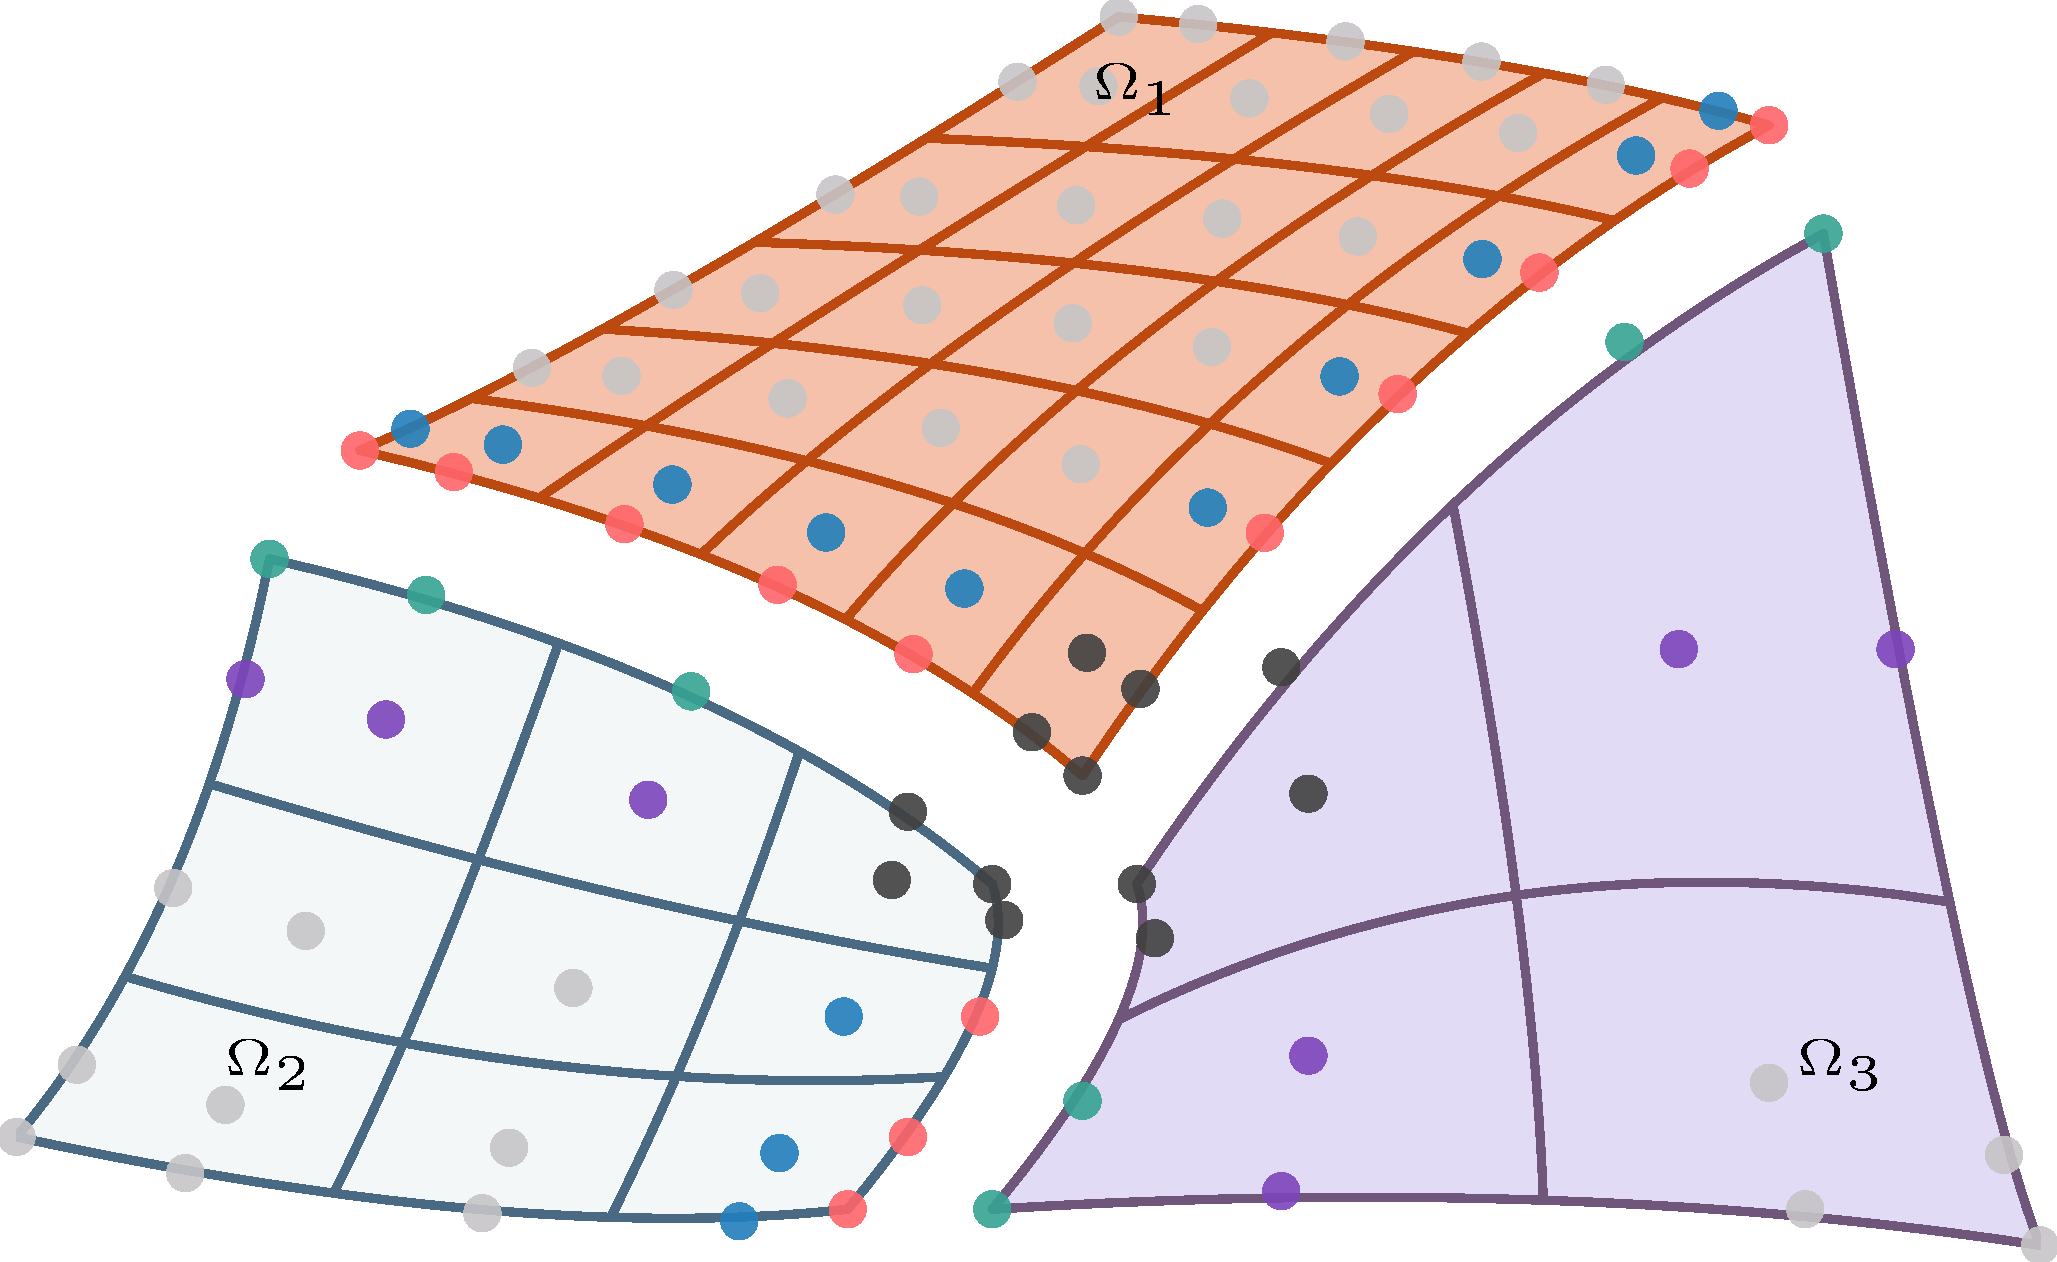
\includegraphics[width=\linewidth]{three_planar_patches}
    \caption{A three-patch planar domain constituted by $\Omega_1$, $\Omega_2$ and $\Omega_3$.}\label{fig:three_planar_patches}
\end{figure}
To generate complex geometries, we need to decompose domain to multiple patches. Unfortunately, we cannot apply directly the results of two-patch coupling to this more general mortar situation. The main issue is the so-called cross points. For a multi-patch decomposition, at least three subdomains meet at an interior crosspoint and several interfaces can share this cross point as a common endpoint (Figure.~\ref{fig:three_planar_patches}). If we use the discretized Lagrange multipliers proposed in the previous section, owing to the presence of cross points, some of the control points will serve as both slave points (indices in $I_1$ and $I_2$) and master points (indices in $I_3$ and $I_4$). Hence, there is no permutation matrices such that the constraint matrix $\mathbf{B}$ can be modified to the form as equation~\eqref{eq:simple_form}, of which the null space can be found in a trivial way. Even more, although the constraint matrices defined on each interfaces are full row rank, the assembled constraint matrix $\mathbf{B}$ may not be full row rank in most cases, which renders the linear system~\eqref{eq:lagrange_multiplier_dicretize} to be rank deficient. As a result, either modifications to the Lagrange multipliers or to the method itself is required so that the proposed method can be generalized to a setting where a domain can be decomposed to an arbitrary number of patches. Before we start this section, we would like to introduce the sixth kind of NURBS basis function that associated with the cross point $v$, as
\begin{enumerate}
    \setcounter{enumi}{5}
    \item The basis function $N_i$ such that $\supp(N_i)\bigcap{v}\neq{}0$, or $\supp(\frac{\partial{}N_i}{\partial\xi})\bigcap{v}\neq{}0$,  or $\supp(\frac{\partial{}N_i}{\partial\eta})\bigcap{v}\neq{}0$ or $\supp(\frac{\partial^2{}N_i}{\partial\xi\partial\eta})\bigcap{v}\neq{}0$, whose indices are in the index set $I_{vi}$. (denoted by black dots in Figure.~\ref{fig:three_planar_patches})
\end{enumerate}
The rest five kinds of NURBS basis function remain the same except their intersection with the sixth kind are excluded, that is
\begin{equation}
    I_k=I_k-I_{vi}\bigcap{}I_k, \quad k\in\{i,ii,\dots,v\}.
\end{equation}
The basis functions in $\mathcal{M}_0^h$ and $\mathcal{M}_1^h$ can be classified as the dual basis functions of the NURBS basis function of the $1^{st}$, $2^{nd}$ and $6^{th}$ kind, respectively. The domains on the two sides of each interface can still be considered as slave and master based on the same rule as for the two-patch coupling case.
\subsection{Cross point modification}
Since using the discretization of Lagrange multipliers proposed for two-patch coupling case directly results in over-constrained constraint matrix $\mathbf{B}$ for the control points round the crosspoints, we can remedy this issue by reducing the dimension of the Lagrange multiplier spaces. Roughly speaking, we have to remove the two degrees of freedom of the Lagrange multiplier spaces associated with each cross point so that the resulted Lagrange multiplier spaces on each interface should have the same dimension as $\mathcal{X}_b^h\vert_{\Omega_s}\bigcap{}H_0^2(\Gamma_{sm})$.\par
\begin{figure}[hbt]
	\centering
    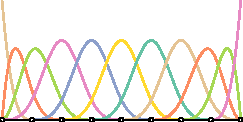
\includegraphics[width=.5\linewidth]{basis_original}\\
    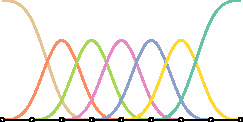
\includegraphics[width=.5\linewidth]{basis_coarse}\\
    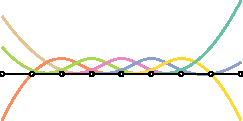
\includegraphics[width=.5\linewidth]{basis_reduce_degree}
	\caption{Quadratic basis functions and their cross point modifications. Top: original quadratic basis functions. Middle: coarsed basis functions. Bottom: degree reduced basis functions}\label{fig:boundary_modification}
\end{figure}
This can be achieved by two ways: we can either coarse the mesh for the Lagrange multiplier in the neighborhood of the cross point, or reduce their polynomial degree in the neighborhood of the cross point. An example for quadratic $1$-D B-spline basis functions is shown in Figure.~\ref{fig:boundary_modification}. The coarsed basis functions are achieved by replacing the first three and last three basis functions by their summations, while we can construct degree reduced basis functions by reduce the polynomial degree of the first and last two elements by one while retaining the inter-element continuity.\par

Although the degree reduction is not a trivial task for dual basis, the summation trick can be applied to coarse dual basis functions. After the coarsen procedure, the dual basis functions associated with the basis functions of $6^{th}$ kind are all eliminated so that no inter-dependencies will happen in the neighborhood of the cross point. We can define a column permutation matrix 
\begin{equation}
    \begin{bmatrix}
        \mathbf{I}_{i}\\
        \mathbf{I}_{ii}\\
        \mathbf{I}_{iii}\\
        \mathbf{I}_{iv}\\
        \mathbf{I}_{vi}\\
        \mathbf{I}_{v}
    \end{bmatrix}=
    \tilde{\mathbf{P}}_c
    \begin{bmatrix}
        \mathbf{I}_1\\
        \mathbf{I}_2\\
        \mathbf{I}_3
    \end{bmatrix}.
\end{equation}
With a suitable row permutation matrix $\tilde{\mathbf{P}}_r$, the constraint matrix $\mathbf{B}$ can be modified as
\begin{equation}
    \tilde{\mathbf{B}}_p:=\tilde{\mathbf{P}}_r\mathbf{B}\tilde{\mathbf{P}}_c^T=
    \begin{bmatrix}
        \mathbf{B}_1^1 & \mathbf{B}_1^2 & \mathbf{B}_1^3 & \mathbf{B}_1^4 & \mathbf{B}_1^6 & \mathbf{0} \\
        \mathbf{0} & \mathbf{B}_2^2 & \mathbf{B}_2^3 & \mathbf{0} & \mathbf{B}_2^6 & \mathbf{0}
    \end{bmatrix},
\end{equation}
with $\mathbf{B}_1^1$ and $\mathbf{B}_2^2$ be identity matrices. Hence, its null space can be found as
\begin{equation}
    \tilde{\mathbf{C}}_p:=\ker(\tilde{\mathbf{B}}_p)=
    \left[\begin{array}{cccc}
      \mathbf{B}_1^2\mathbf{B}_2^3-\mathbf{B}_1^3 & -\mathbf{B}_1^4 & -\mathbf{B}_1^6 & \mathbf{0} \\ 
      -\mathbf{B}_2^3 & \mathbf{0} & -\mathbf{B}_2^6 & \mathbf{0} \\ \hdashline[2pt/2pt]
       \multicolumn{4}{c}{\multirow{3}{*}{\raisebox{0mm}{\scalebox{1.5}{$\mathbf{I}$}}}}\\
       & & & 
    \end{array}\right].
\end{equation}
Although the boundary modification by coarsening eliminates the inter-dependency in the neighborhood of cross points, numerical tests demonstrate sub-optimality.  
\subsection{Explicitly solve the null space}
Instead of modifying the Lagrange multipliers, we can solve the null space of the over-constrained constraint matrix $\mathbf{B}$ directly. Seveal matrix factorization methods can be used to solve the null space, including LU, QR, SVD. For example, a rank-revealing QR factorization over a rank-deficiency constraint matrix $\mathbf{B}$ yields
\begin{equation}
    \mathbf{B}\mathbf{P}=
    \mathbf{Q}
    \begin{bmatrix}
        \mathbf{R}_1 & \mathbf{R}_2 \\
        \mathbf{0} & \mathbf{0}
    \end{bmatrix}
\end{equation}
where $\mathbf{P}$ is a permutation matrix, $\mathbf{Q}$ is an unitary matrix, $\mathbf{R}_1$ is a upper triangular matrix and $\mathbf{R}_2$ is a rectangular matrix. The null space can be taken as 
\begin{equation}
    \ker(\mathbf{B})=
    \mathbf{P}
    \begin{bmatrix}
        -\mathbf{R}_1^{-1}\mathbf{R}_2\\
        \mathbf{I}
    \end{bmatrix}.\label{eq:direct_kernel}
\end{equation}
However, this requires a factorization of the entire constraint matrix $\mathbf{B}$ and we fail to utilize the advantage of the \Bezier dual basis. Even more, the sparsity of the constrained stiffness matrix might be impacted as the inverse of $\mathbf{R}_1$ is a dense matrix. This type of global factorization has been utilized for patch coupling problem in~\cite{coox_robust_2017, coox2017flexible, dornisch2017dual}.\par
Instead of solving the null space directly, we will localize the constraint to each cross point and solve the null space of a localized linear system. For the constraint matrix $\mathbf{B}$ constructed by the Lagrange multipliers without modification, we assume there exist a row permutation matrix $\hat{\mathbf{P}}_r$ such that
\begin{equation}
    \hat{\mathbf{B}}_p:=\hat{\mathbf{P}}_r\mathbf{B}\tilde{\mathbf{P}}_c^T=
    \begin{bmatrix}
        {\mathbf{B}}_1\\  \hdashline[2pt/2pt]
        {\mathbf{B}}_2
    \end{bmatrix}
    =
    \begin{bmatrix}
        \mathbf{B}_6^1 & \mathbf{B}_6^2 & \mathbf{B}_6^3 & \mathbf{B}_6^4 & \mathbf{B}_6^6 & \mathbf{0} \\ \hdashline[2pt/2pt]
        \mathbf{B}_1^1 & \mathbf{B}_1^2 & \mathbf{B}_1^3 & \mathbf{B}_1^4 & \mathbf{B}_1^6 & \mathbf{0} \\
        \mathbf{0} & \mathbf{B}_2^2 & \mathbf{B}_2^3 & \mathbf{0} & \mathbf{B}_2^6 & \mathbf{0}
    \end{bmatrix},
\end{equation}
with $\mathbf{B}_1^1$ and $\mathbf{B}_2^2$ be identity matrices. $\mathbf{B}_1$ consists of constraints relevant to cross point while $\mathbf{B}_2$ consists of constraints relevant to intersections. \par
The null space of ${\mathbf{B}}_2$ can be found as
\begin{equation}
    \mathbf{C}_2:=\ker({\mathbf{B}}_2)=
    \left[\begin{array}{cccc}
      \mathbf{B}_1^2\mathbf{B}_2^3-\mathbf{B}_1^3 & -\mathbf{B}_1^4 & -\mathbf{B}_1^6 & \mathbf{0} \\ 
      -\mathbf{B}_2^3 & \mathbf{0} & -\mathbf{B}_2^6 & \mathbf{0} \\ \hdashline[2pt/2pt]
       \multicolumn{4}{c}{\multirow{3}{*}{\raisebox{0mm}{\scalebox{1.5}{$\mathbf{I}$}}}}\\
       & & & 
    \end{array}\right].
\end{equation}
\begin{figure}[hbt]
	\centering
    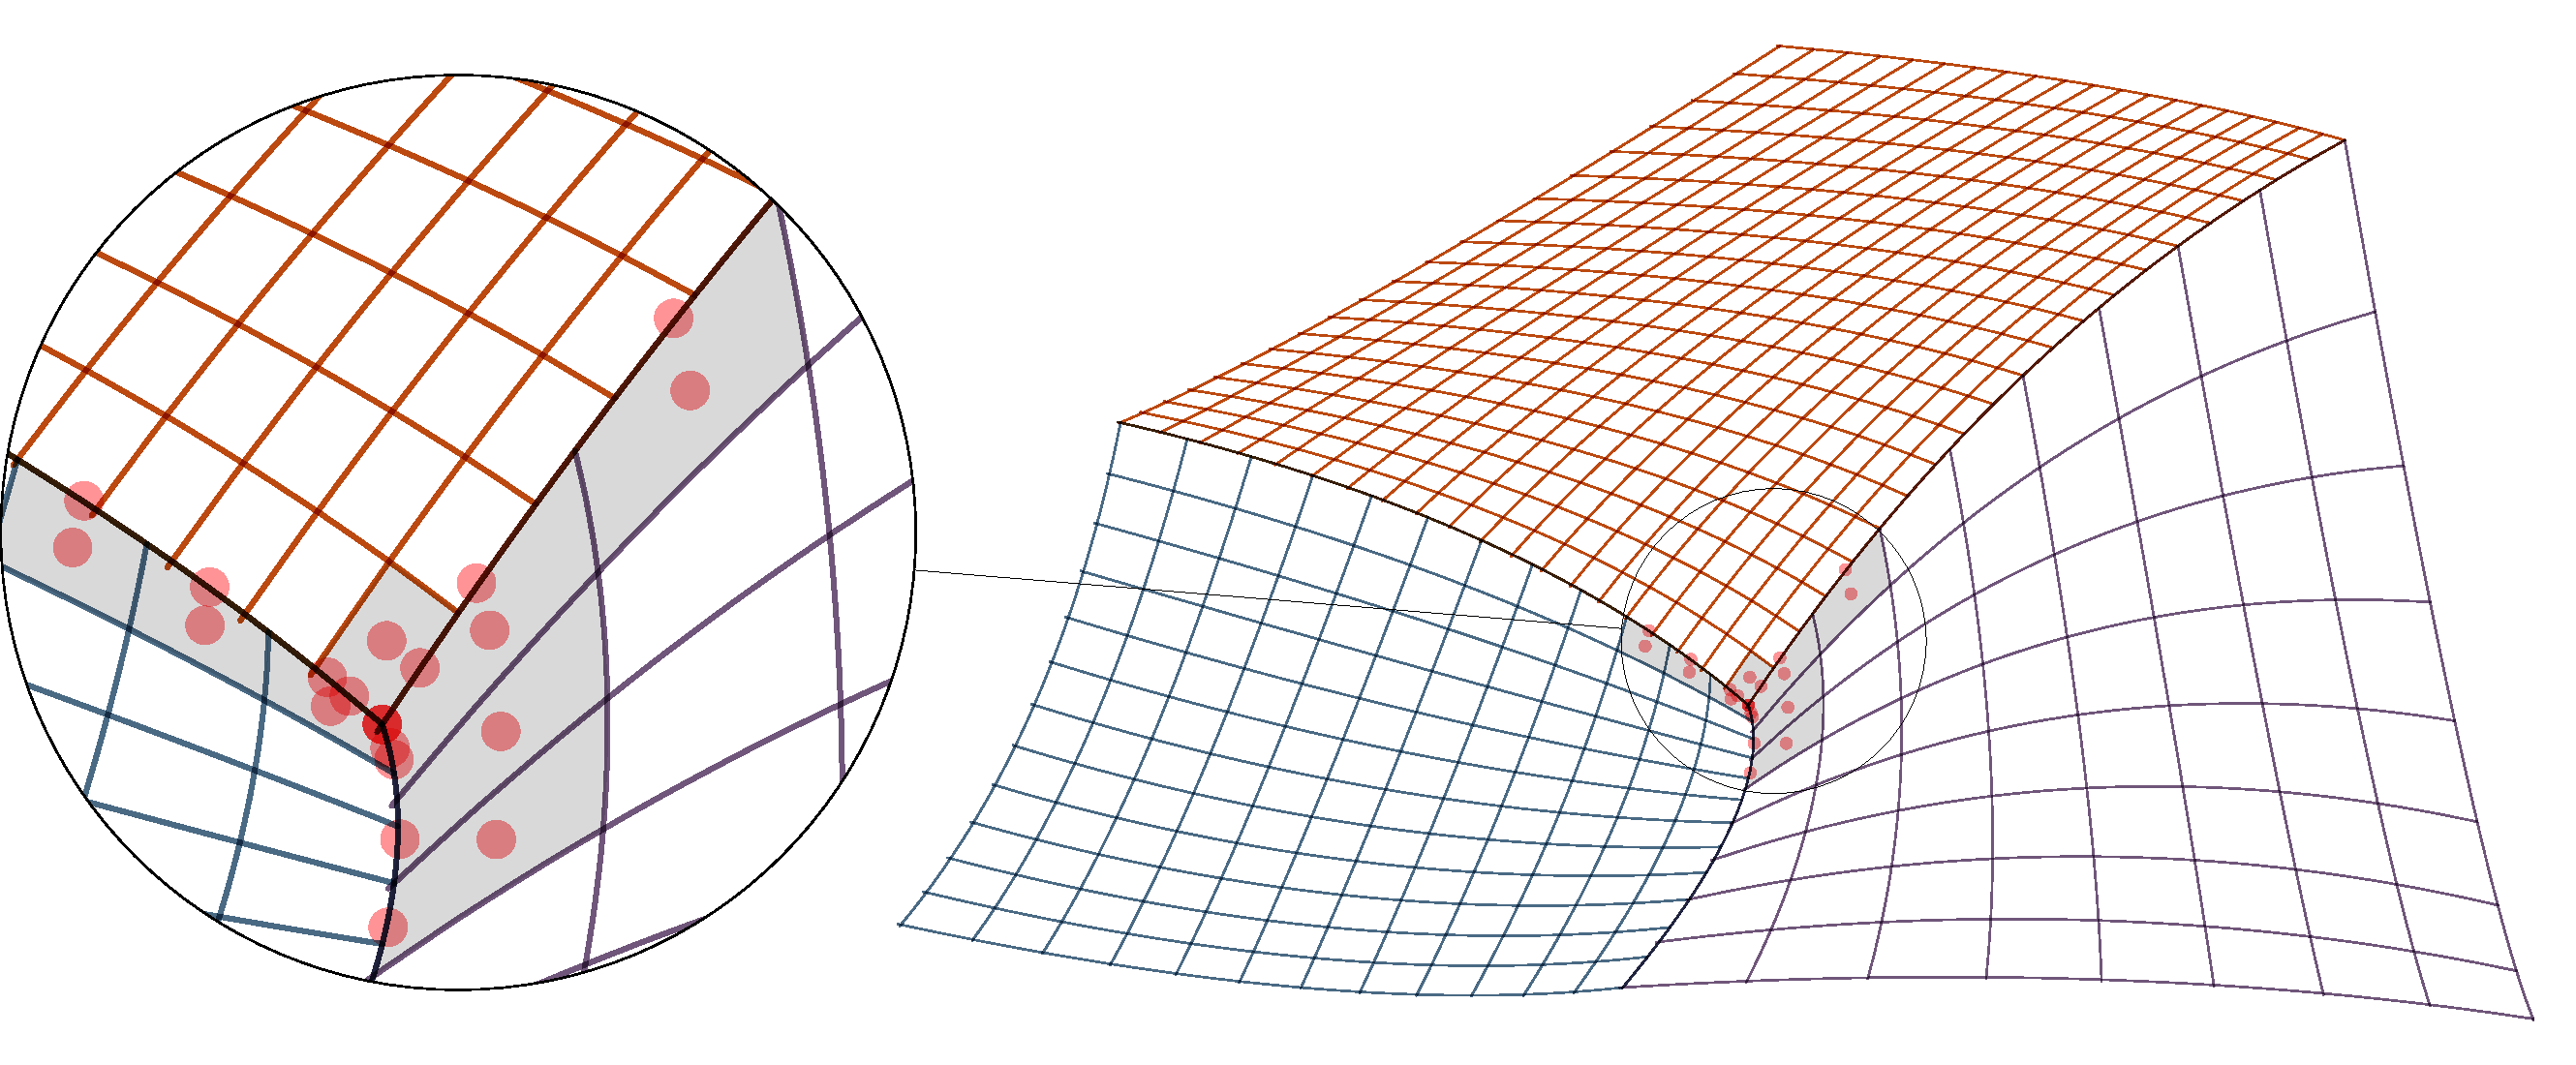
\includegraphics[width=\linewidth]{mesh_spy}
	\caption{Control points (red) involved in crosspoint constraints ($\mathbf{B}_1$).}\label{fig:cross_point_dof}
\end{figure}
Due to the inclusion $\hat{\mathbf{C}}_p:=\ker(\hat{\mathbf{B}}_p)\subset{\ker({\mathbf{B}}_2)}$, we can construct $\hat{\mathbf{C}}_p$ by solving $\ker(\mathbf{B}_1\mathbf{C}_2)$. Since dual basis functions have compact support, $\mathbf{B}_1$ and $\mathbf{C}_2$ are all sparse matrices (control points involved in $\mathbf{B}_1$ are demonstrated in Figure.~\ref{fig:cross_point_dof}). We can split the columns of $\mathbf{C}_2$ into two matrices, as
\begin{align}
    \begin{split}
        \mathbf{C}_2^1&:=\{v\in\mathbf{C}_2\colon{\mathbf{B}_1v\neq{0}}\},\\
        \mathbf{C}_2^2&:=\{v\in\mathbf{C}_2\colon{\mathbf{B}_1v={0}}\}.
    \end{split}
\end{align}
Such a split can be defined a priori, based on the discretization of each patch. A demonstration of the split is givin in Figure.~\ref{fig:overlap_nonoverlap}. Note that $\mathbf{C}_2^2\subset\hat{\mathbf{C}}_p$, $\hat{\mathbf{C}}_p$ can be written as
\begin{equation}
    \hat{\mathbf{C}}_p=
    \begin{bmatrix}
        \mathbf{C}_2^1\ker(\bar{\mathbf{B}}_p) & \mathbf{C}_2^2
    \end{bmatrix}, \text{ with } \bar{\mathbf{B}}_p=\mathbf{B}_1\mathbf{C}_2^1.\label{eq:local_kernel}
\end{equation}
\begin{figure}[hbt]
	\centering
    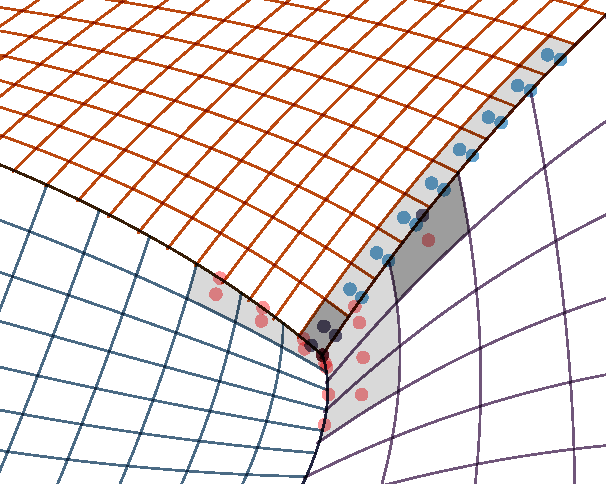
\includegraphics[width=.47\linewidth]{trim_overlap}
    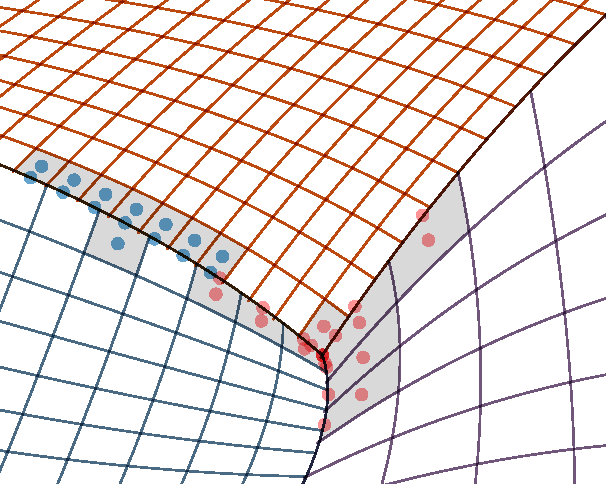
\includegraphics[width=.47\linewidth]{trim_nonoverlap}
	\caption{Control points of basis functions (blue) defined by columns of $\mathbf{C}_2$. Left: Basis classified to $\mathbf{C}_2^1$; Right: Basis classified to $\mathbf{C}_2^2$}\label{fig:overlap_nonoverlap}
\end{figure}
Compared with the constraint matrix $\mathbf{B}$ whose size increases as we refine the mesh, the row size of $\bar{\mathbf{B}}_p$ is fixed and its column size is fixed after certain refinement. A comparison of the size of matrix $\mathbf{B}$ and matrix $\bar{\mathbf{B}}_p$ as a function of the degrees of freedom is given in Figure.~\ref{fig:size_evolution} for the three-patch coupling in Figure.~\ref{fig:three_planar_patches} with $2^{nd}$ order B-spline basis functions. As can be seen, the size of $\mathbf{B}$ grows rapidly as the mesh being refined. The computational cost of directly solving its kernel will be very expensive. However, owing to the compact support of dual basis function, we can transfer a global, size-varying problem (fractorization on $\mathbf{B}$) to a local, size-fixed problem (factorization on $\bar{\mathbf{B}}_p$), and the problem size is very small ($12\times{24}$ for this case).\par

\begin{figure}[hbt]
	\centering
    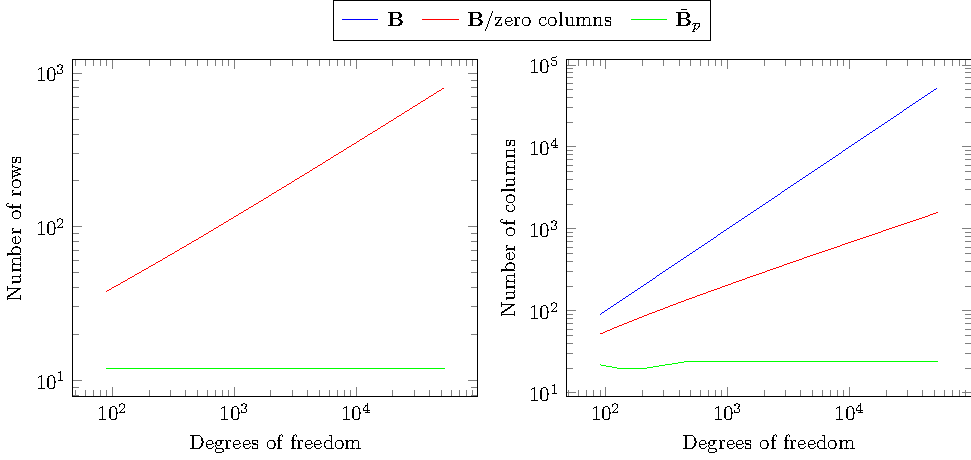
\includegraphics[width=\linewidth]{size_vs_dof}
	\caption{The change of matrix size of $\mathbf{B}$, $\mathbf{B}$ with zero columns being removed, and $\bar{\mathbf{B}}_p$, as a function of the degrees of freedom. The constraint matrix $\mathbf{B}$ is formulated for the three-patch coupling in Figure.~\ref{fig:three_planar_patches} with $2^{nd}$ order B-spline basis functions.}\label{fig:size_evolution}
\end{figure}

A graphical comparison of the sparity patterns among standard Lagrange multiplier with global factorization, \Bezier dual basis with global factorization and \Bezier dual basis with local factorization is given in Figure.~\ref{fig:sparity_pattern}. As expected, the standard method yields the lowest sparsity, while \Bezier dual basis with local factorization yields the highest sparsity ($40\%$ sparser). Meanwhile, the \Bezier dual basis does not significantly improve the sparsity if a global factorization is applied to construct $\mathcal{K}_b^h$. Moreover, a global factorization yeilds entries with very small absolute values ($\leq{}10^{-14}$), especially for the constraint matrix formed by \Bezier dual basis, while all entries are away from zero for the local factorization. 

\begin{figure}[htb]
    \centering
    \begin{tabular}{cp{4cm}p{4cm}p{4cm}}
        \scriptsize\rotatebox[origin=c]{90}{Original} &
        \raisebox{-0.5\height}{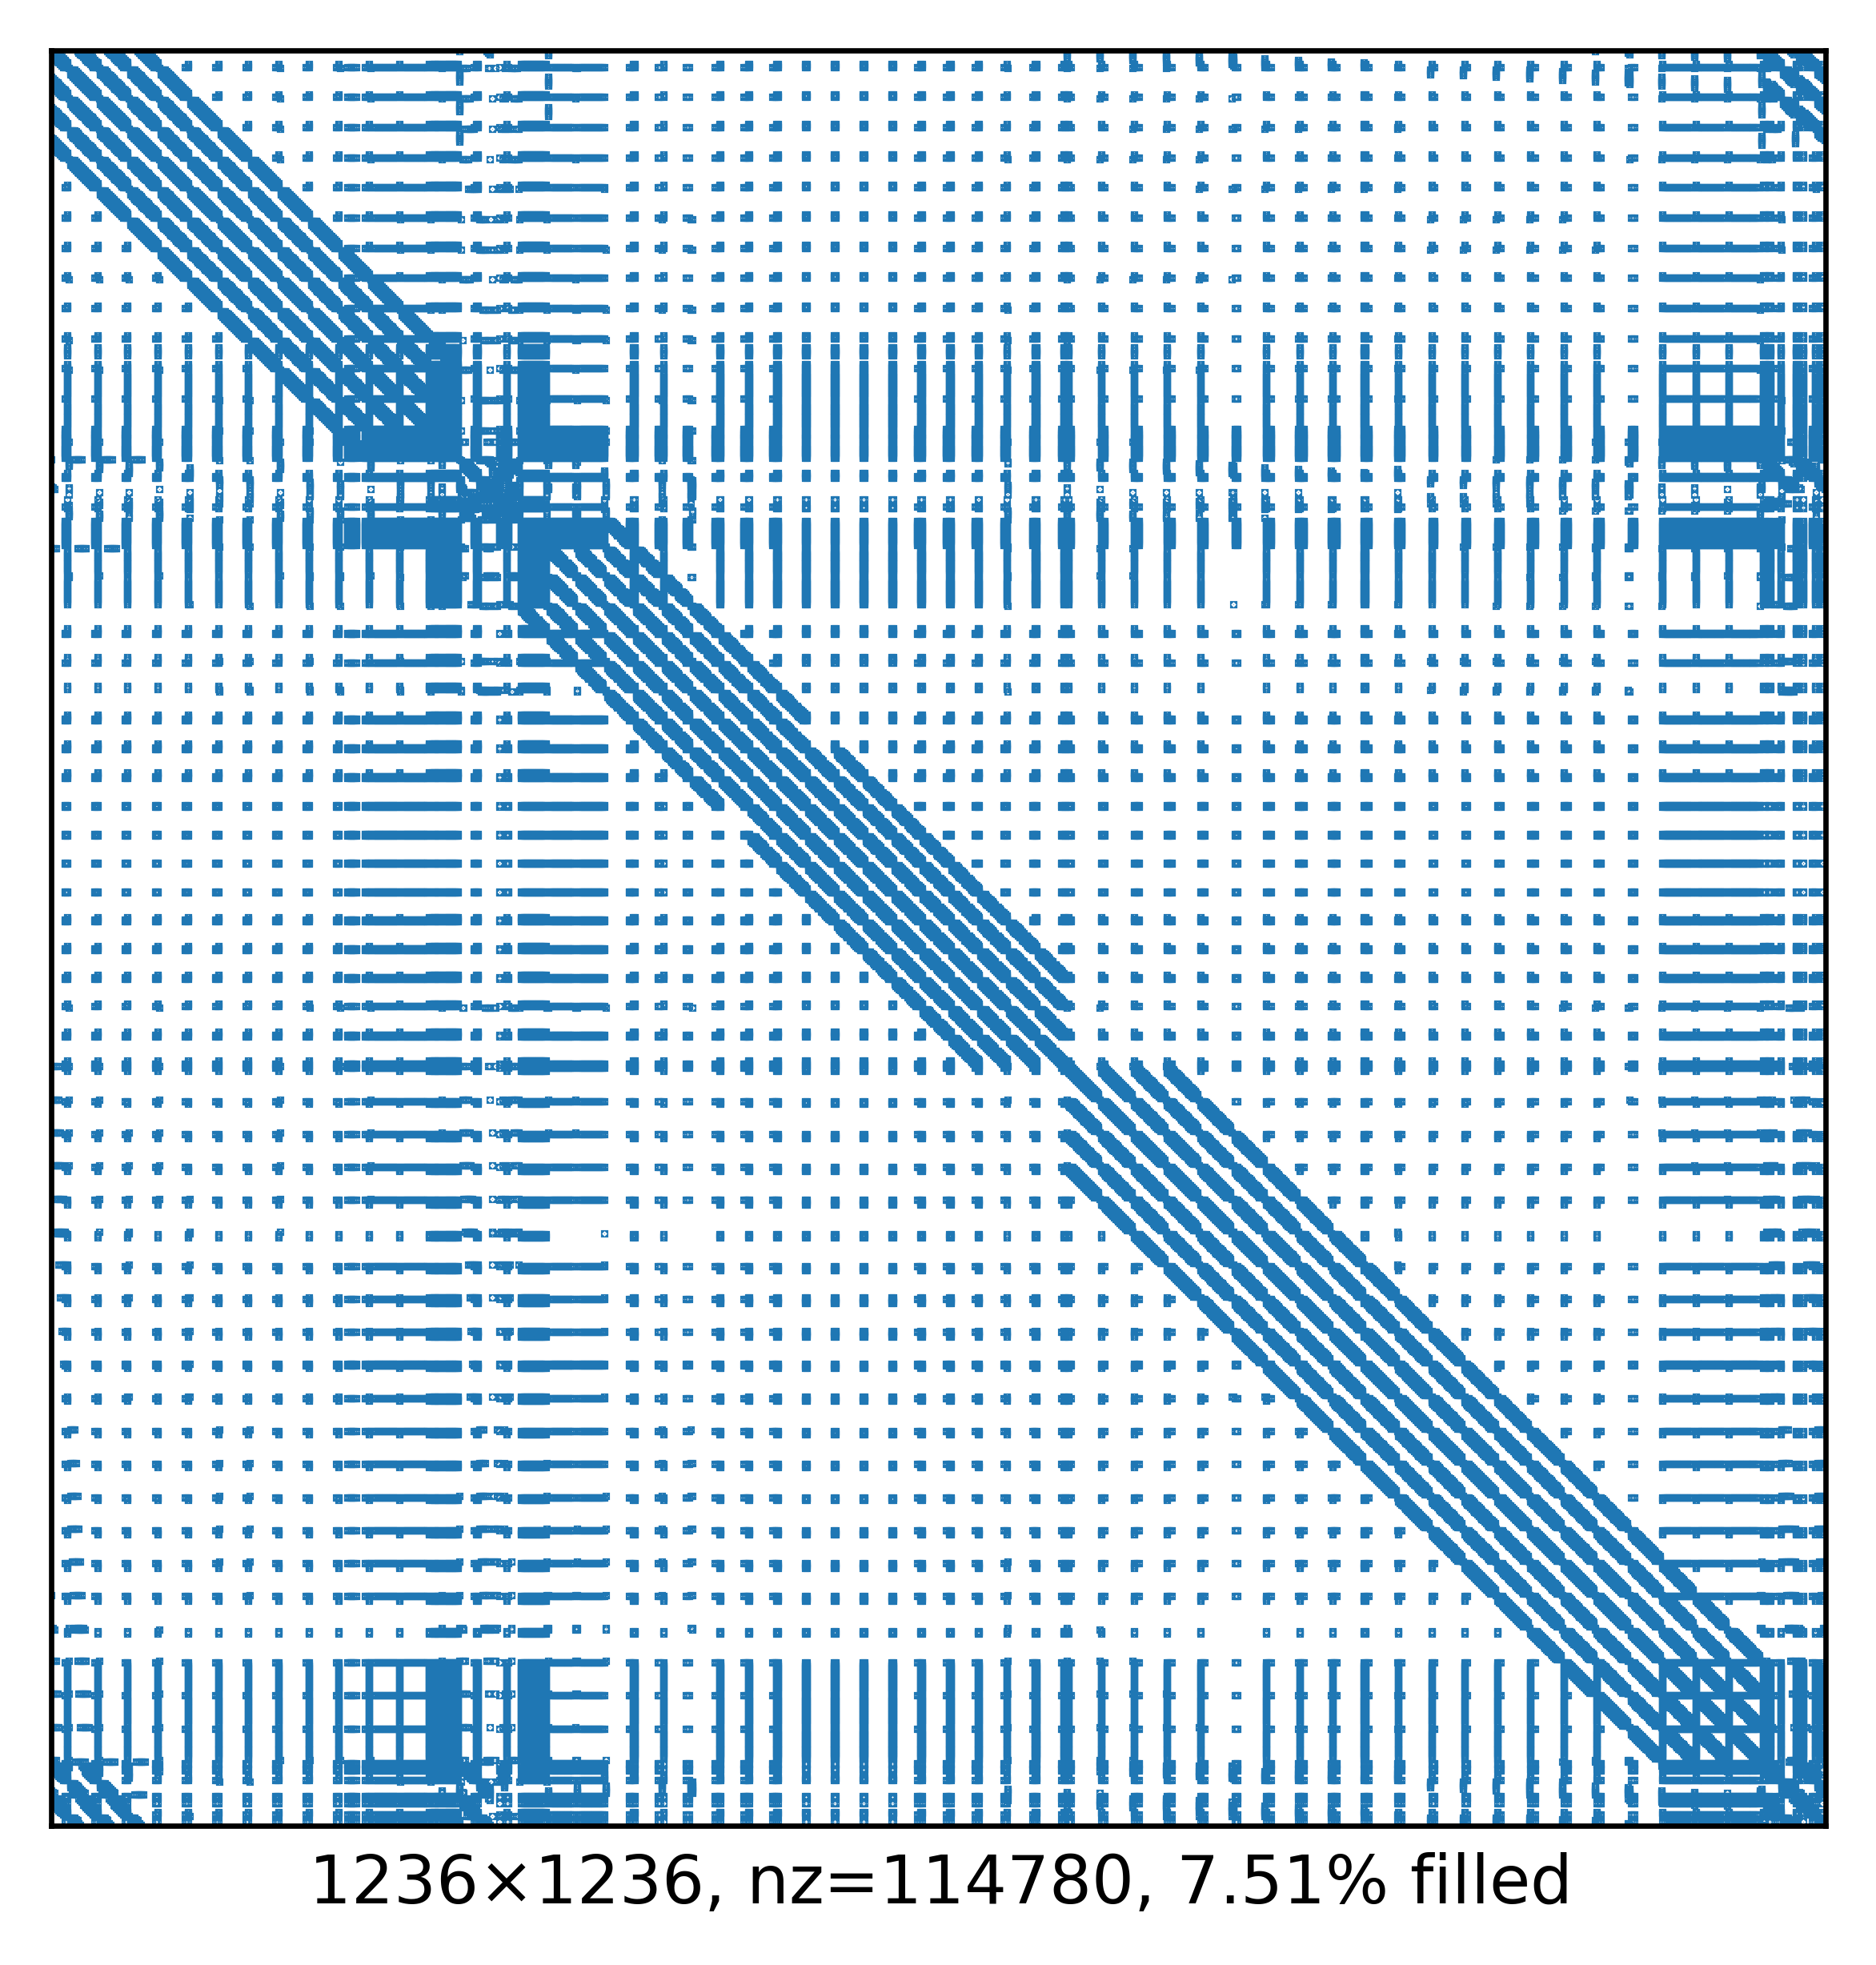
\includegraphics[width=.3\textwidth]{direct1.png}} &
        \raisebox{-0.5\height}{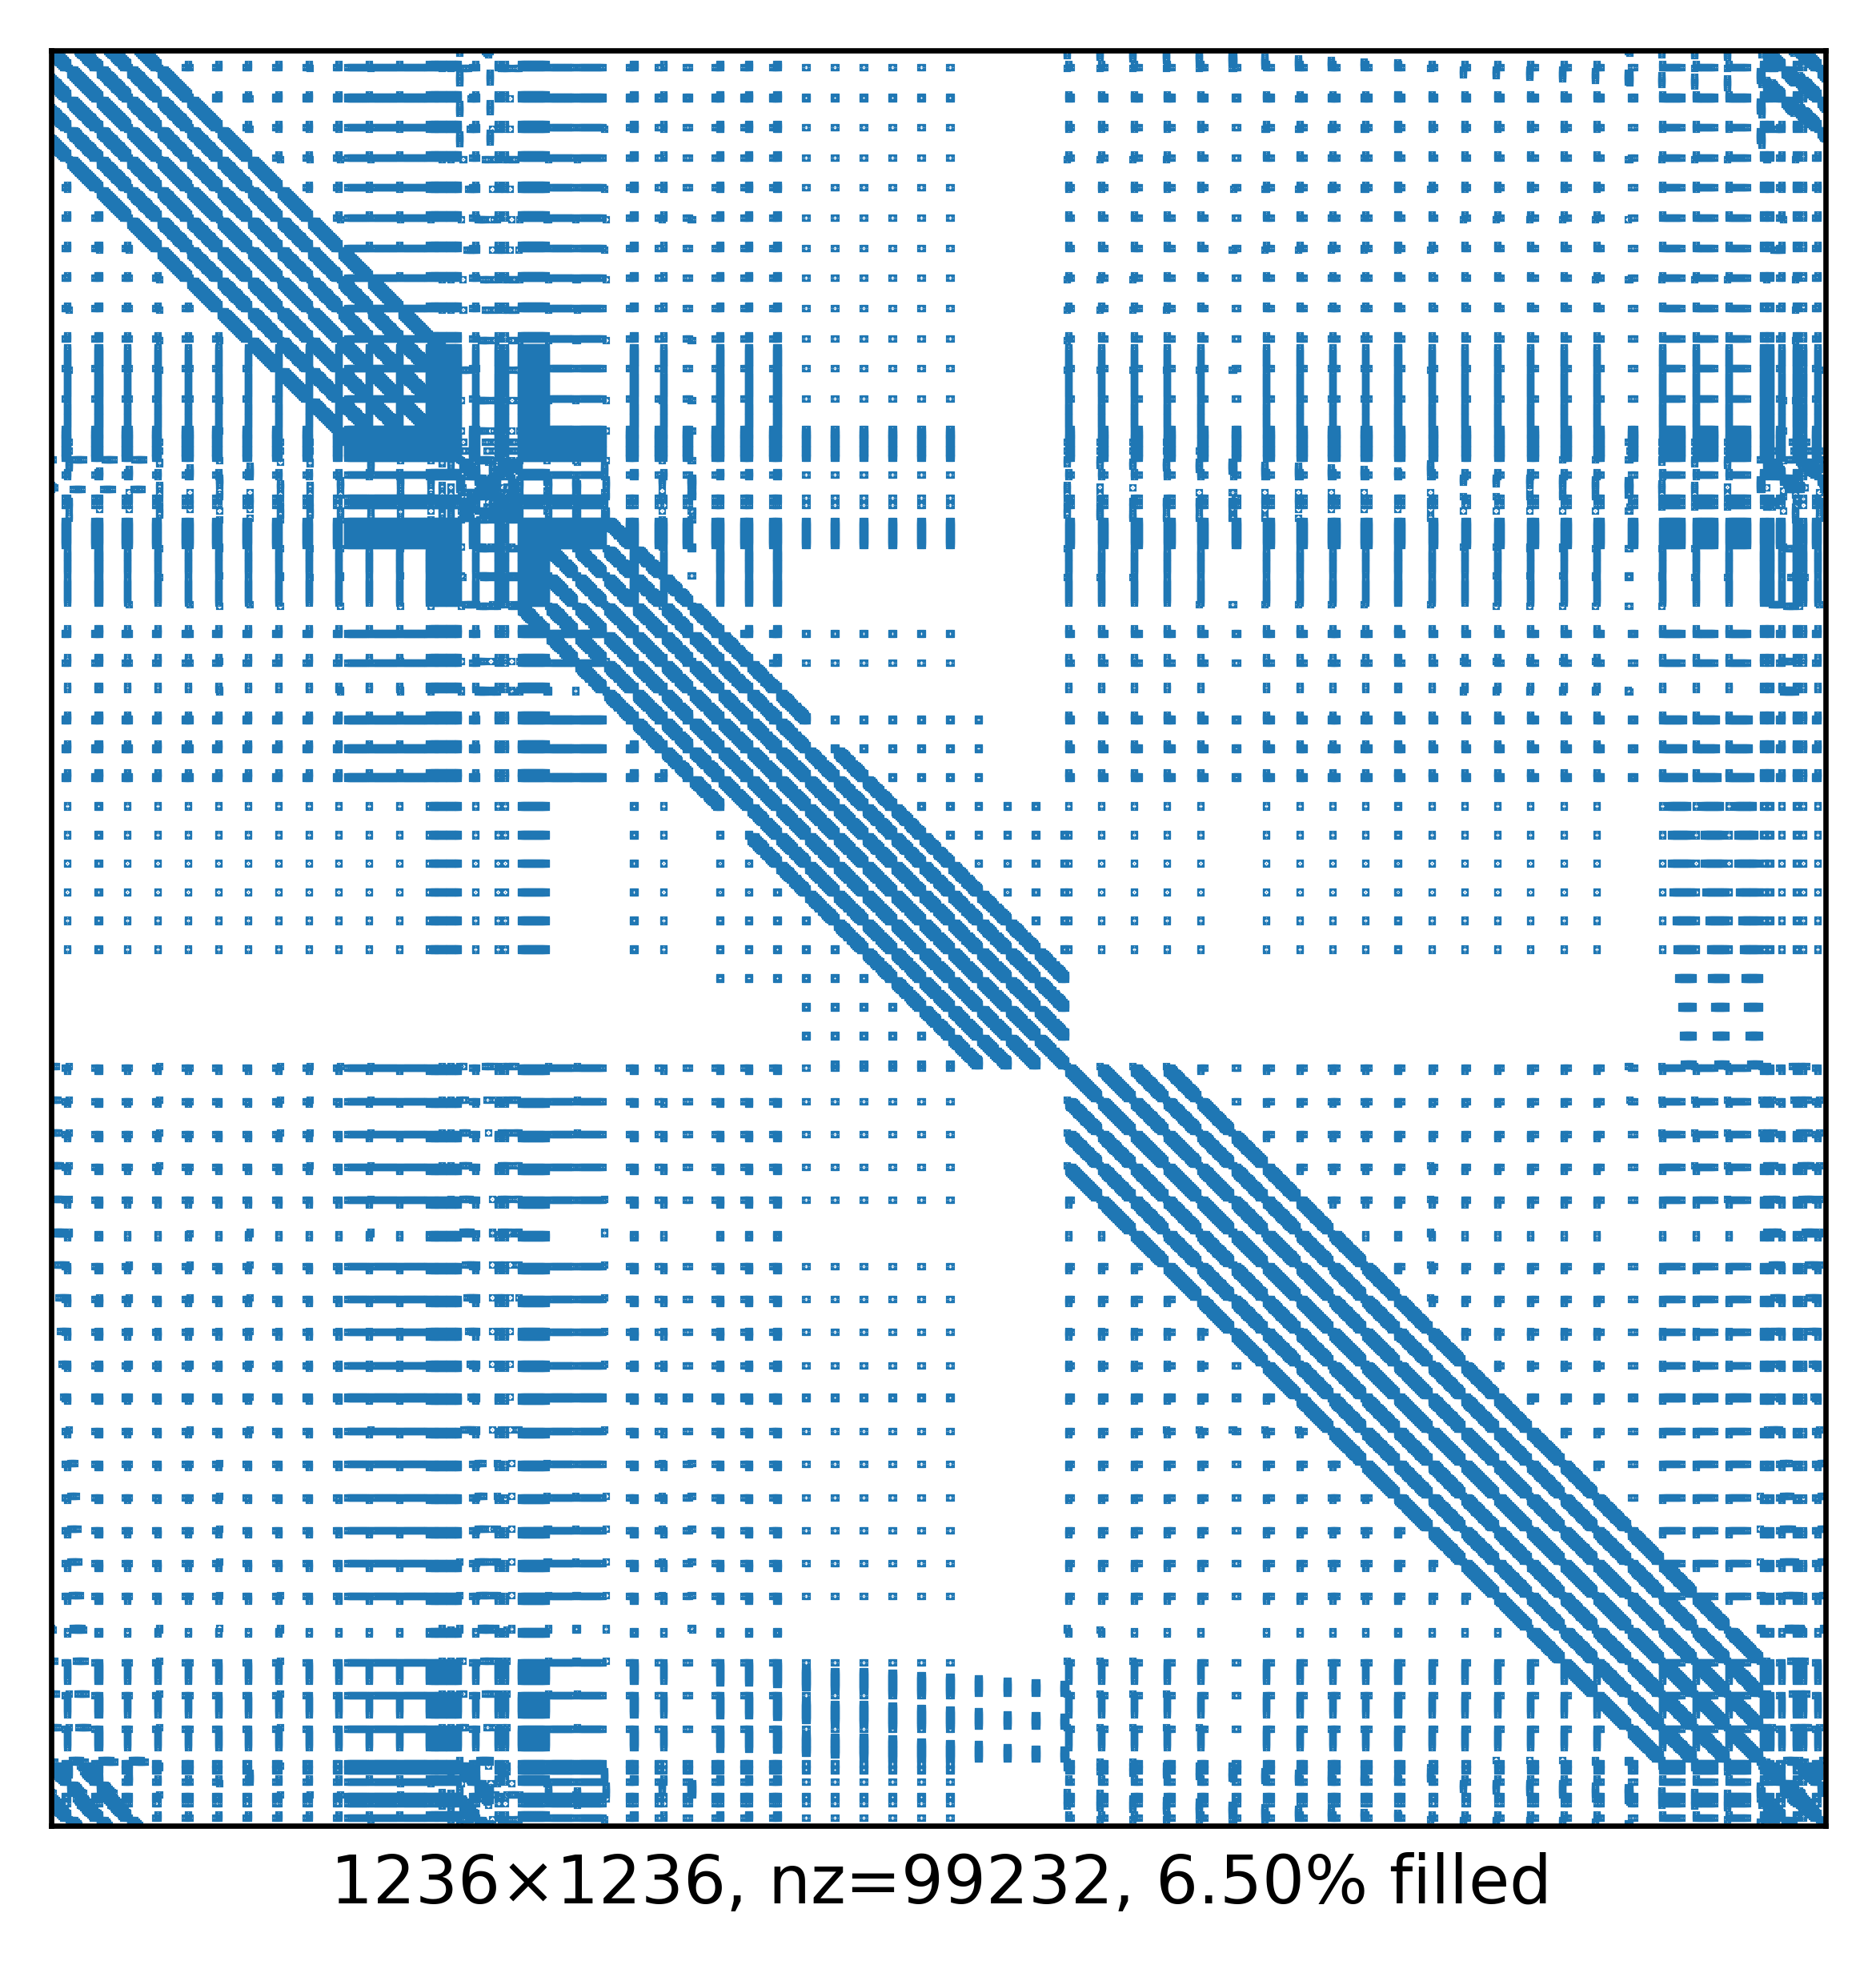
\includegraphics[width=.3\textwidth]{direct.png}} &
        \raisebox{-0.5\height}{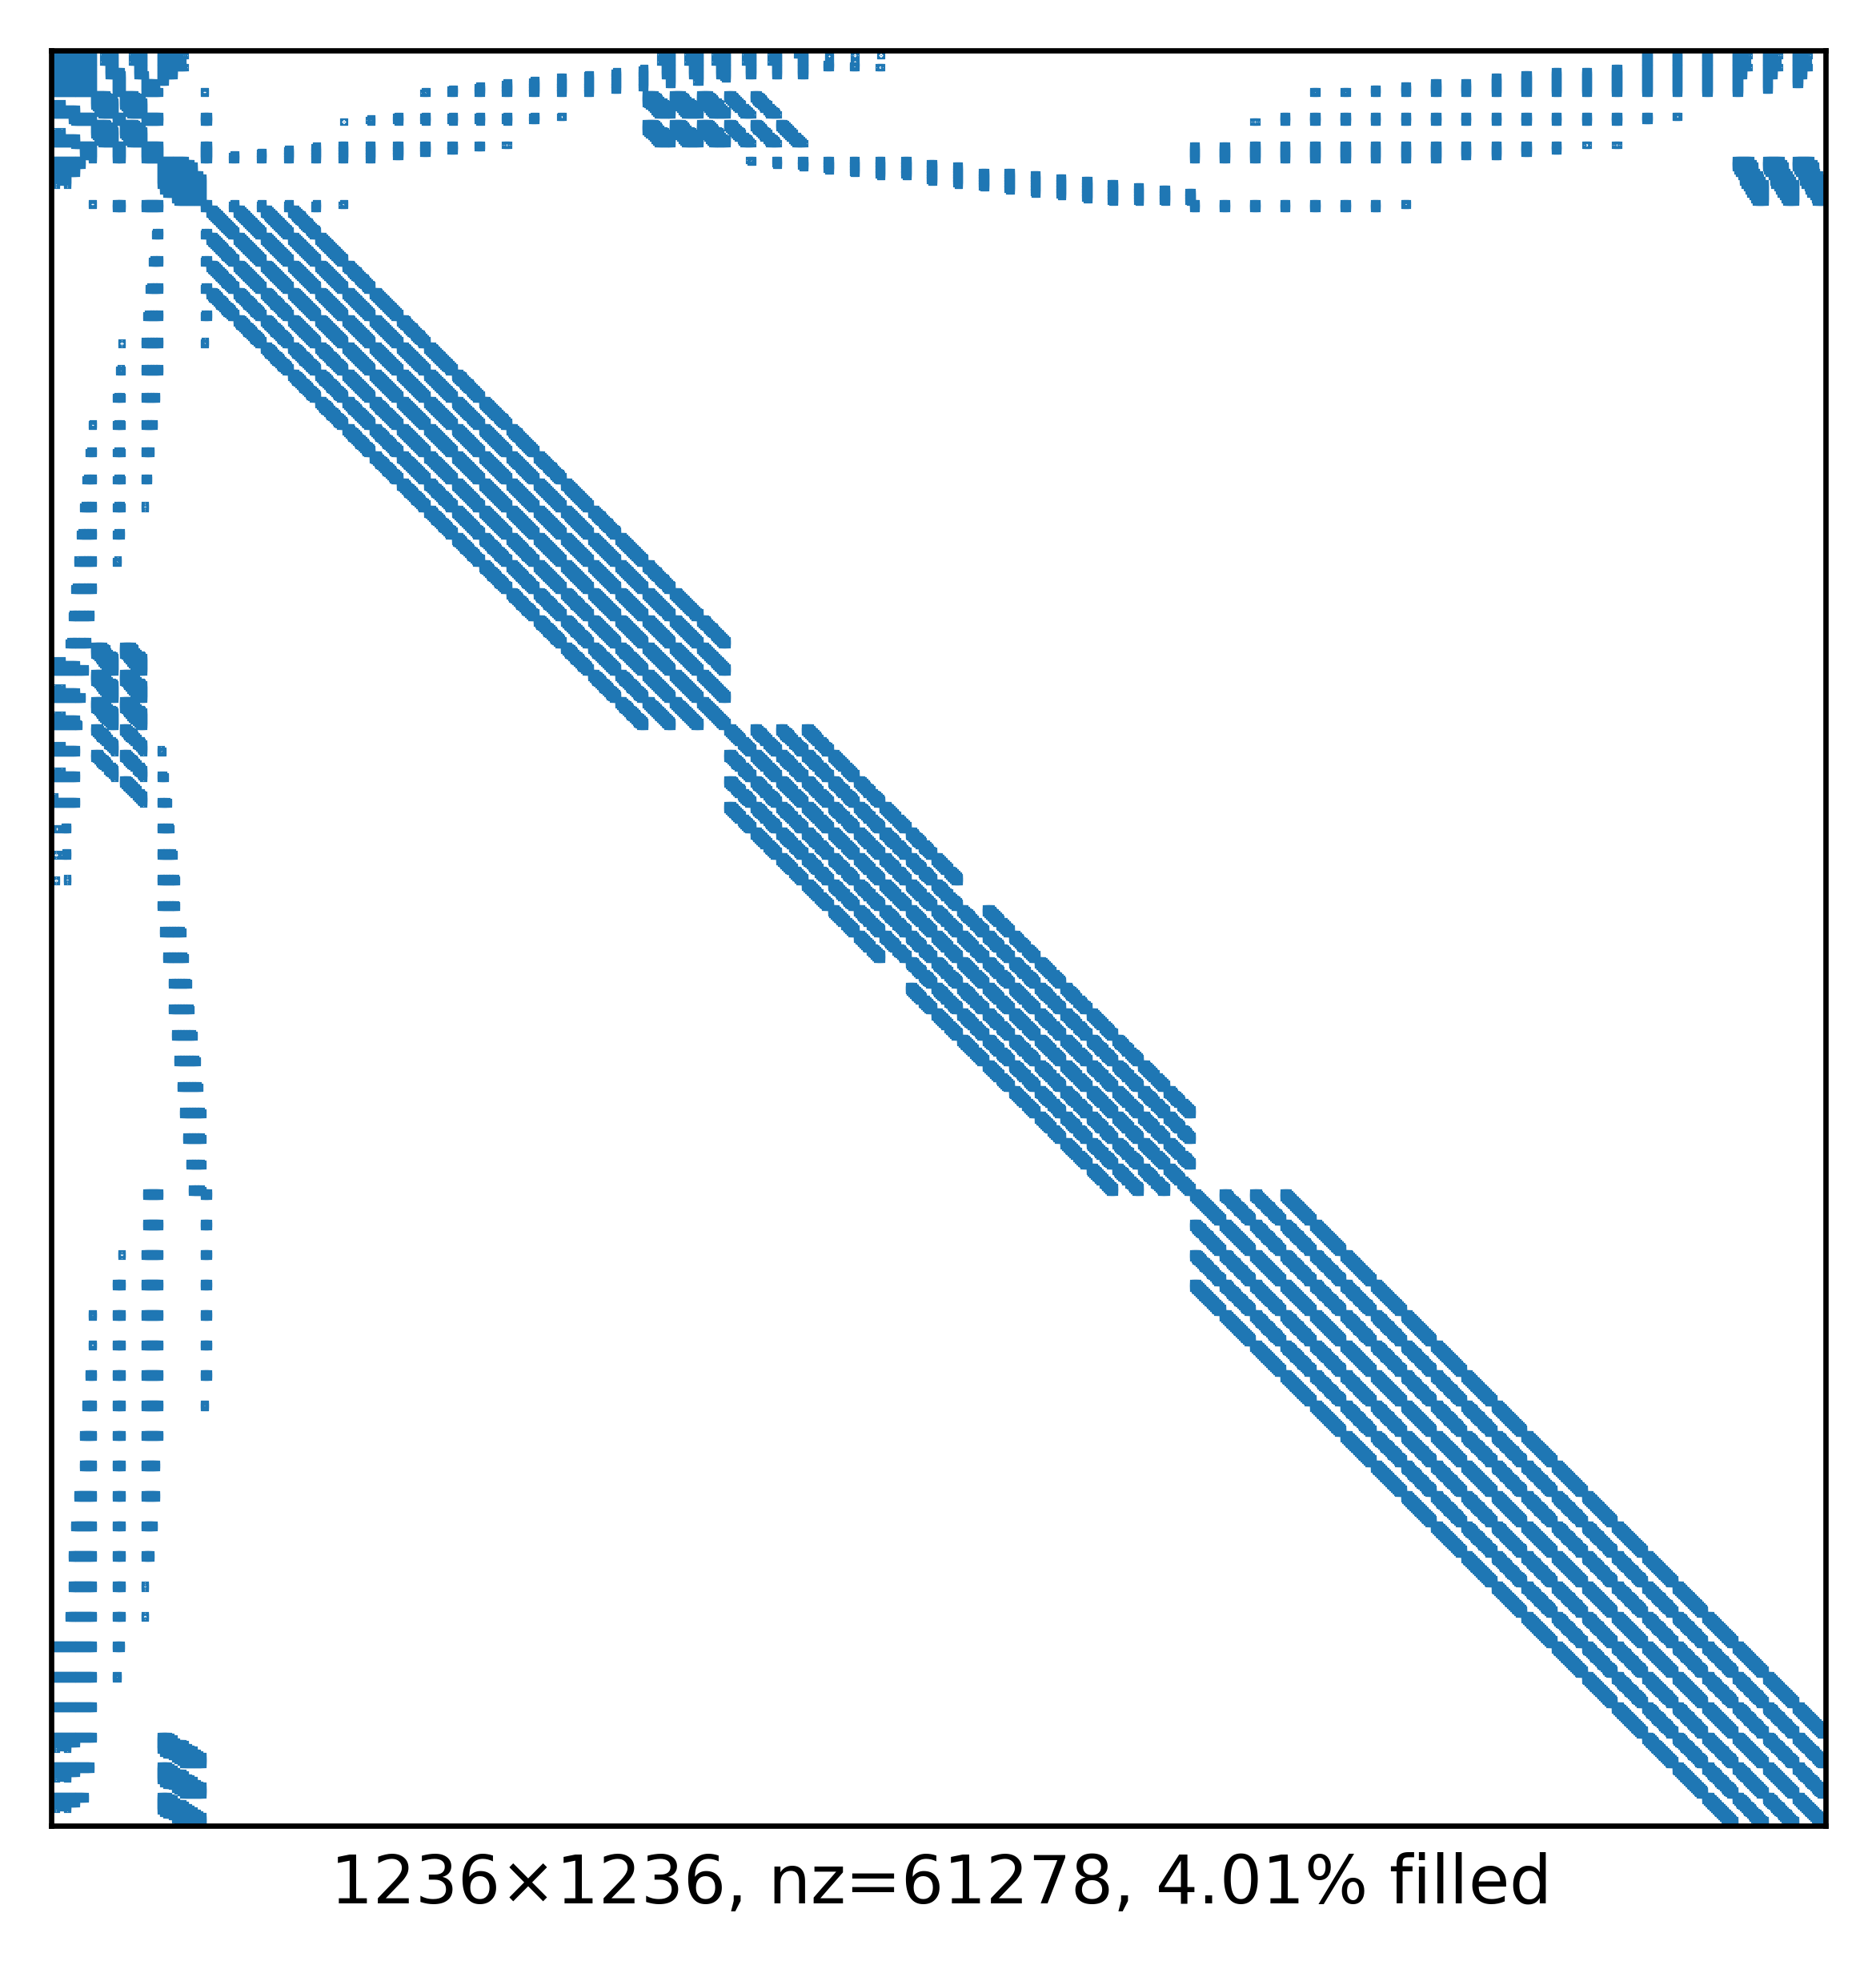
\includegraphics[width=.3\textwidth]{proposed.png}}\\

        \scriptsize\rotatebox[origin=c]{90}{Pruned} &
        \raisebox{-0.5\height}{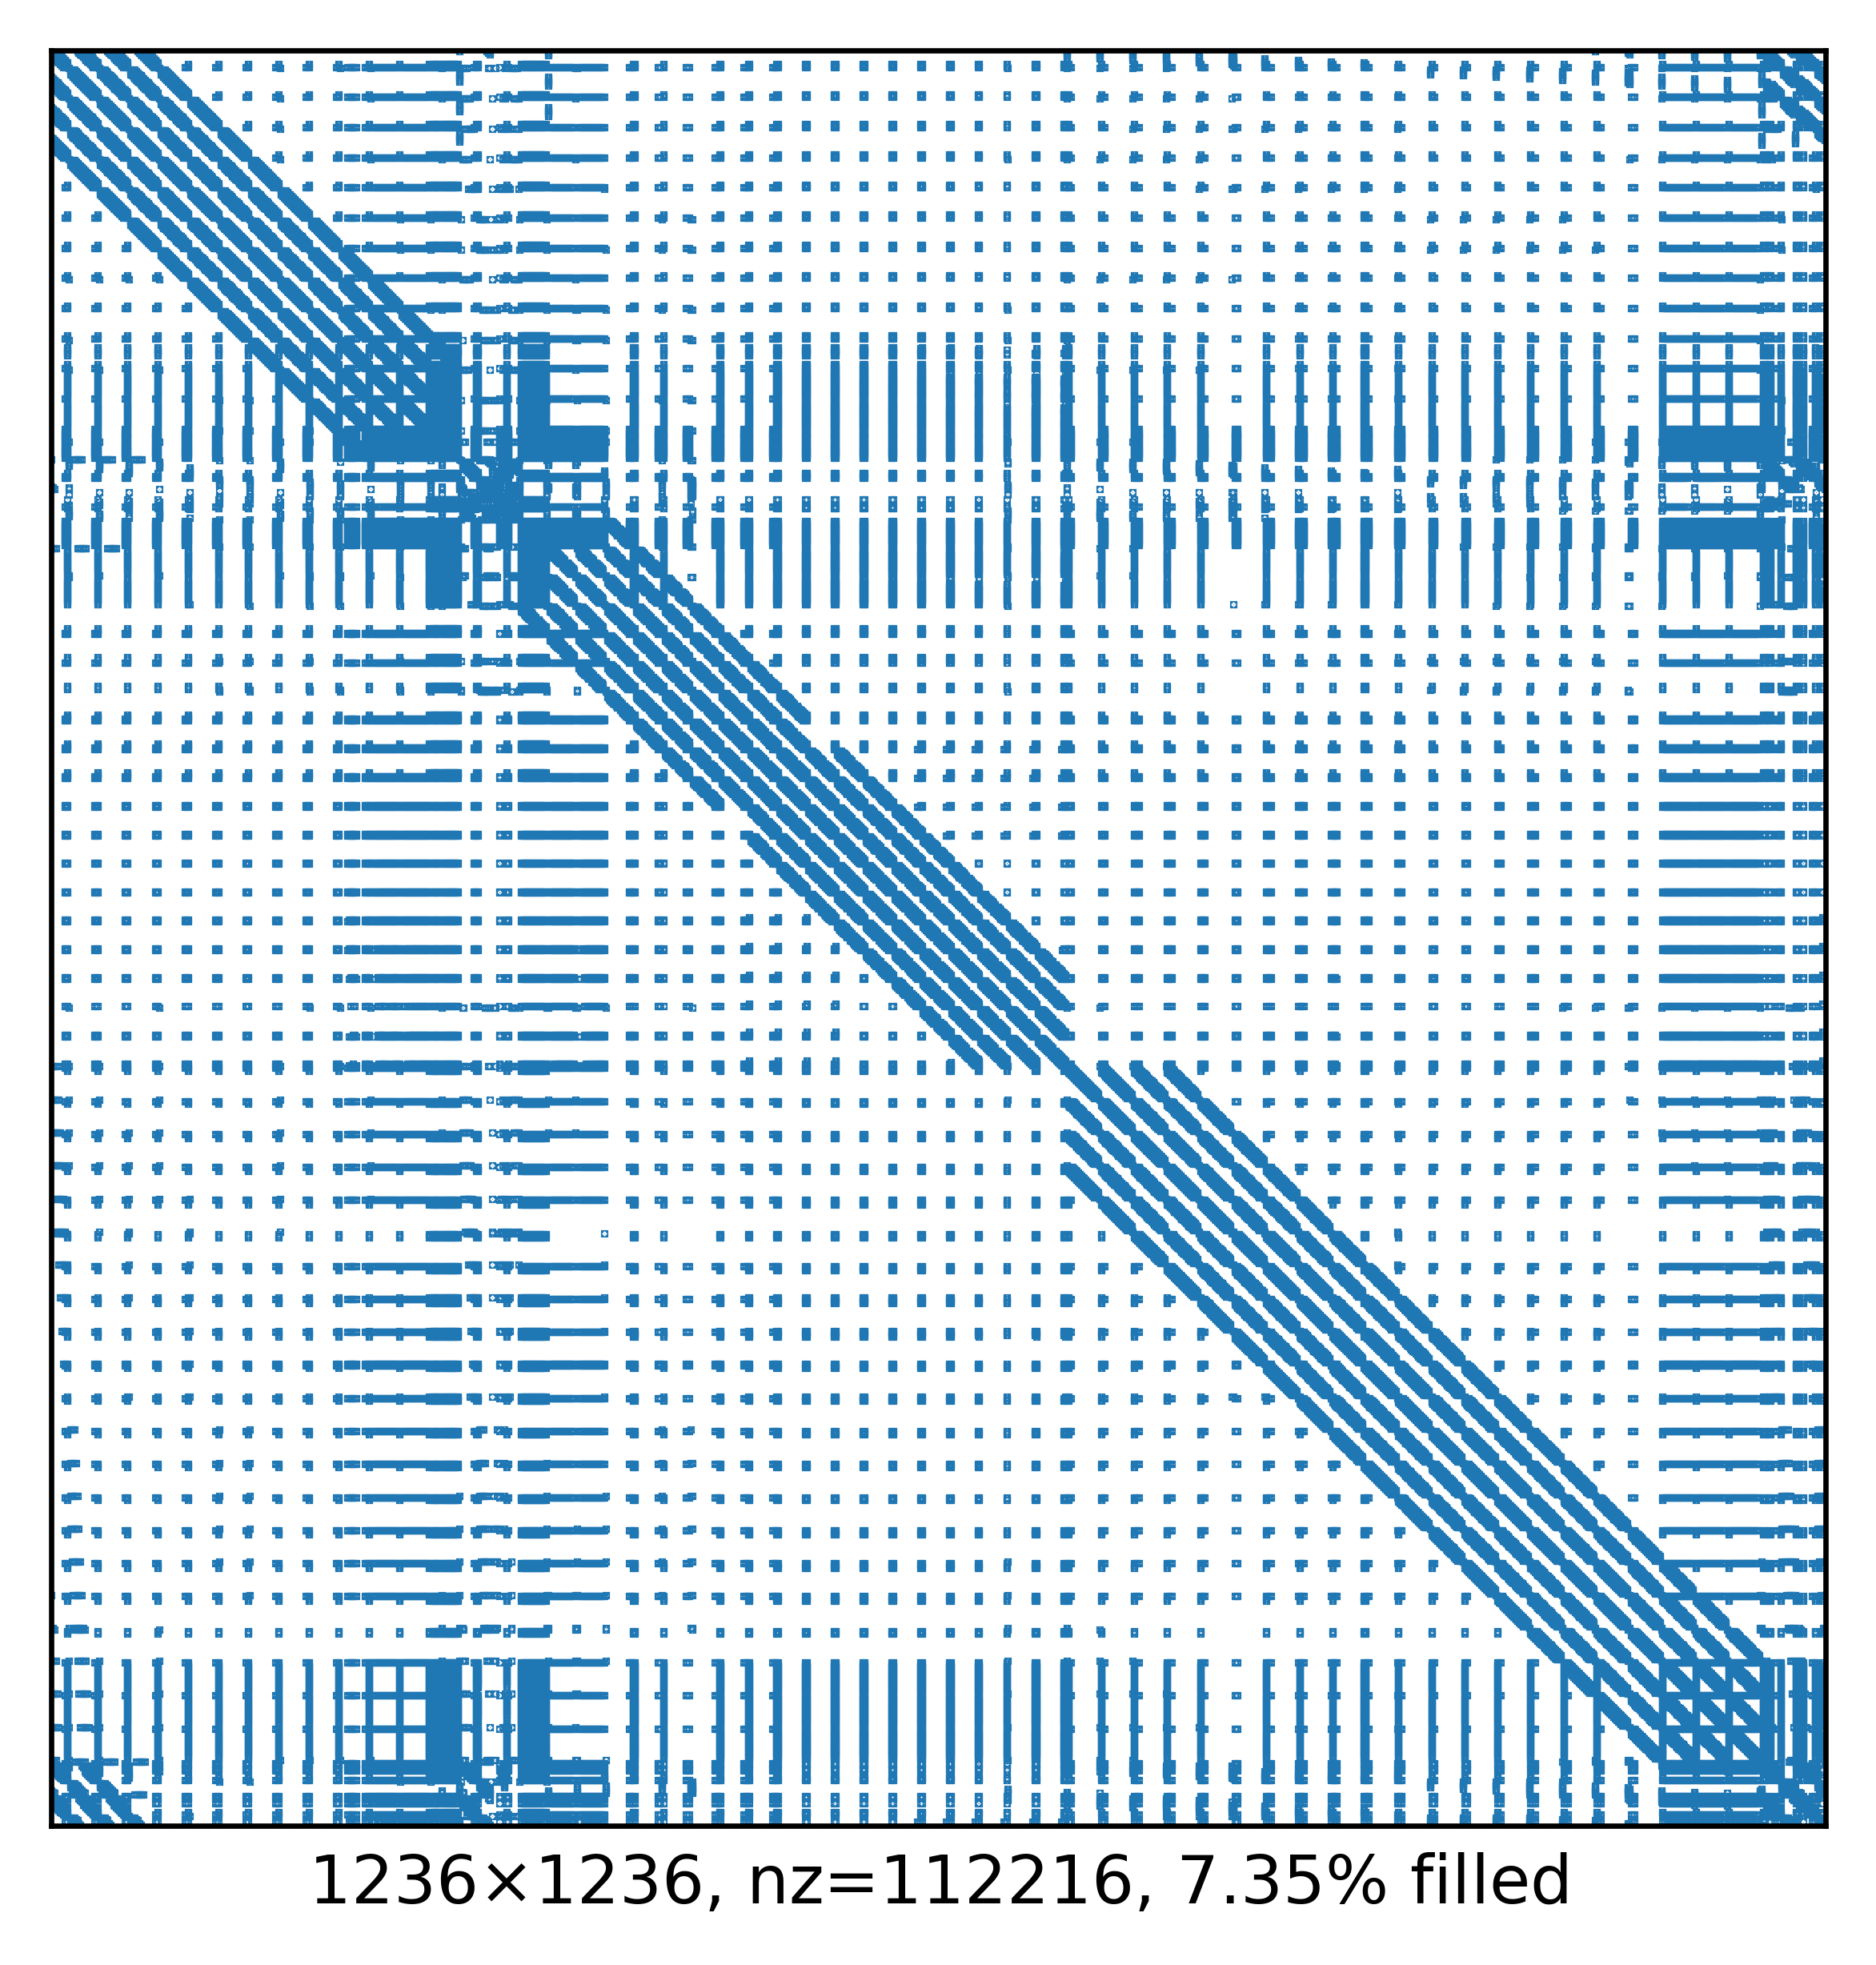
\includegraphics[width=.3\textwidth]{direct1_filtered.png}} &
        \raisebox{-0.5\height}{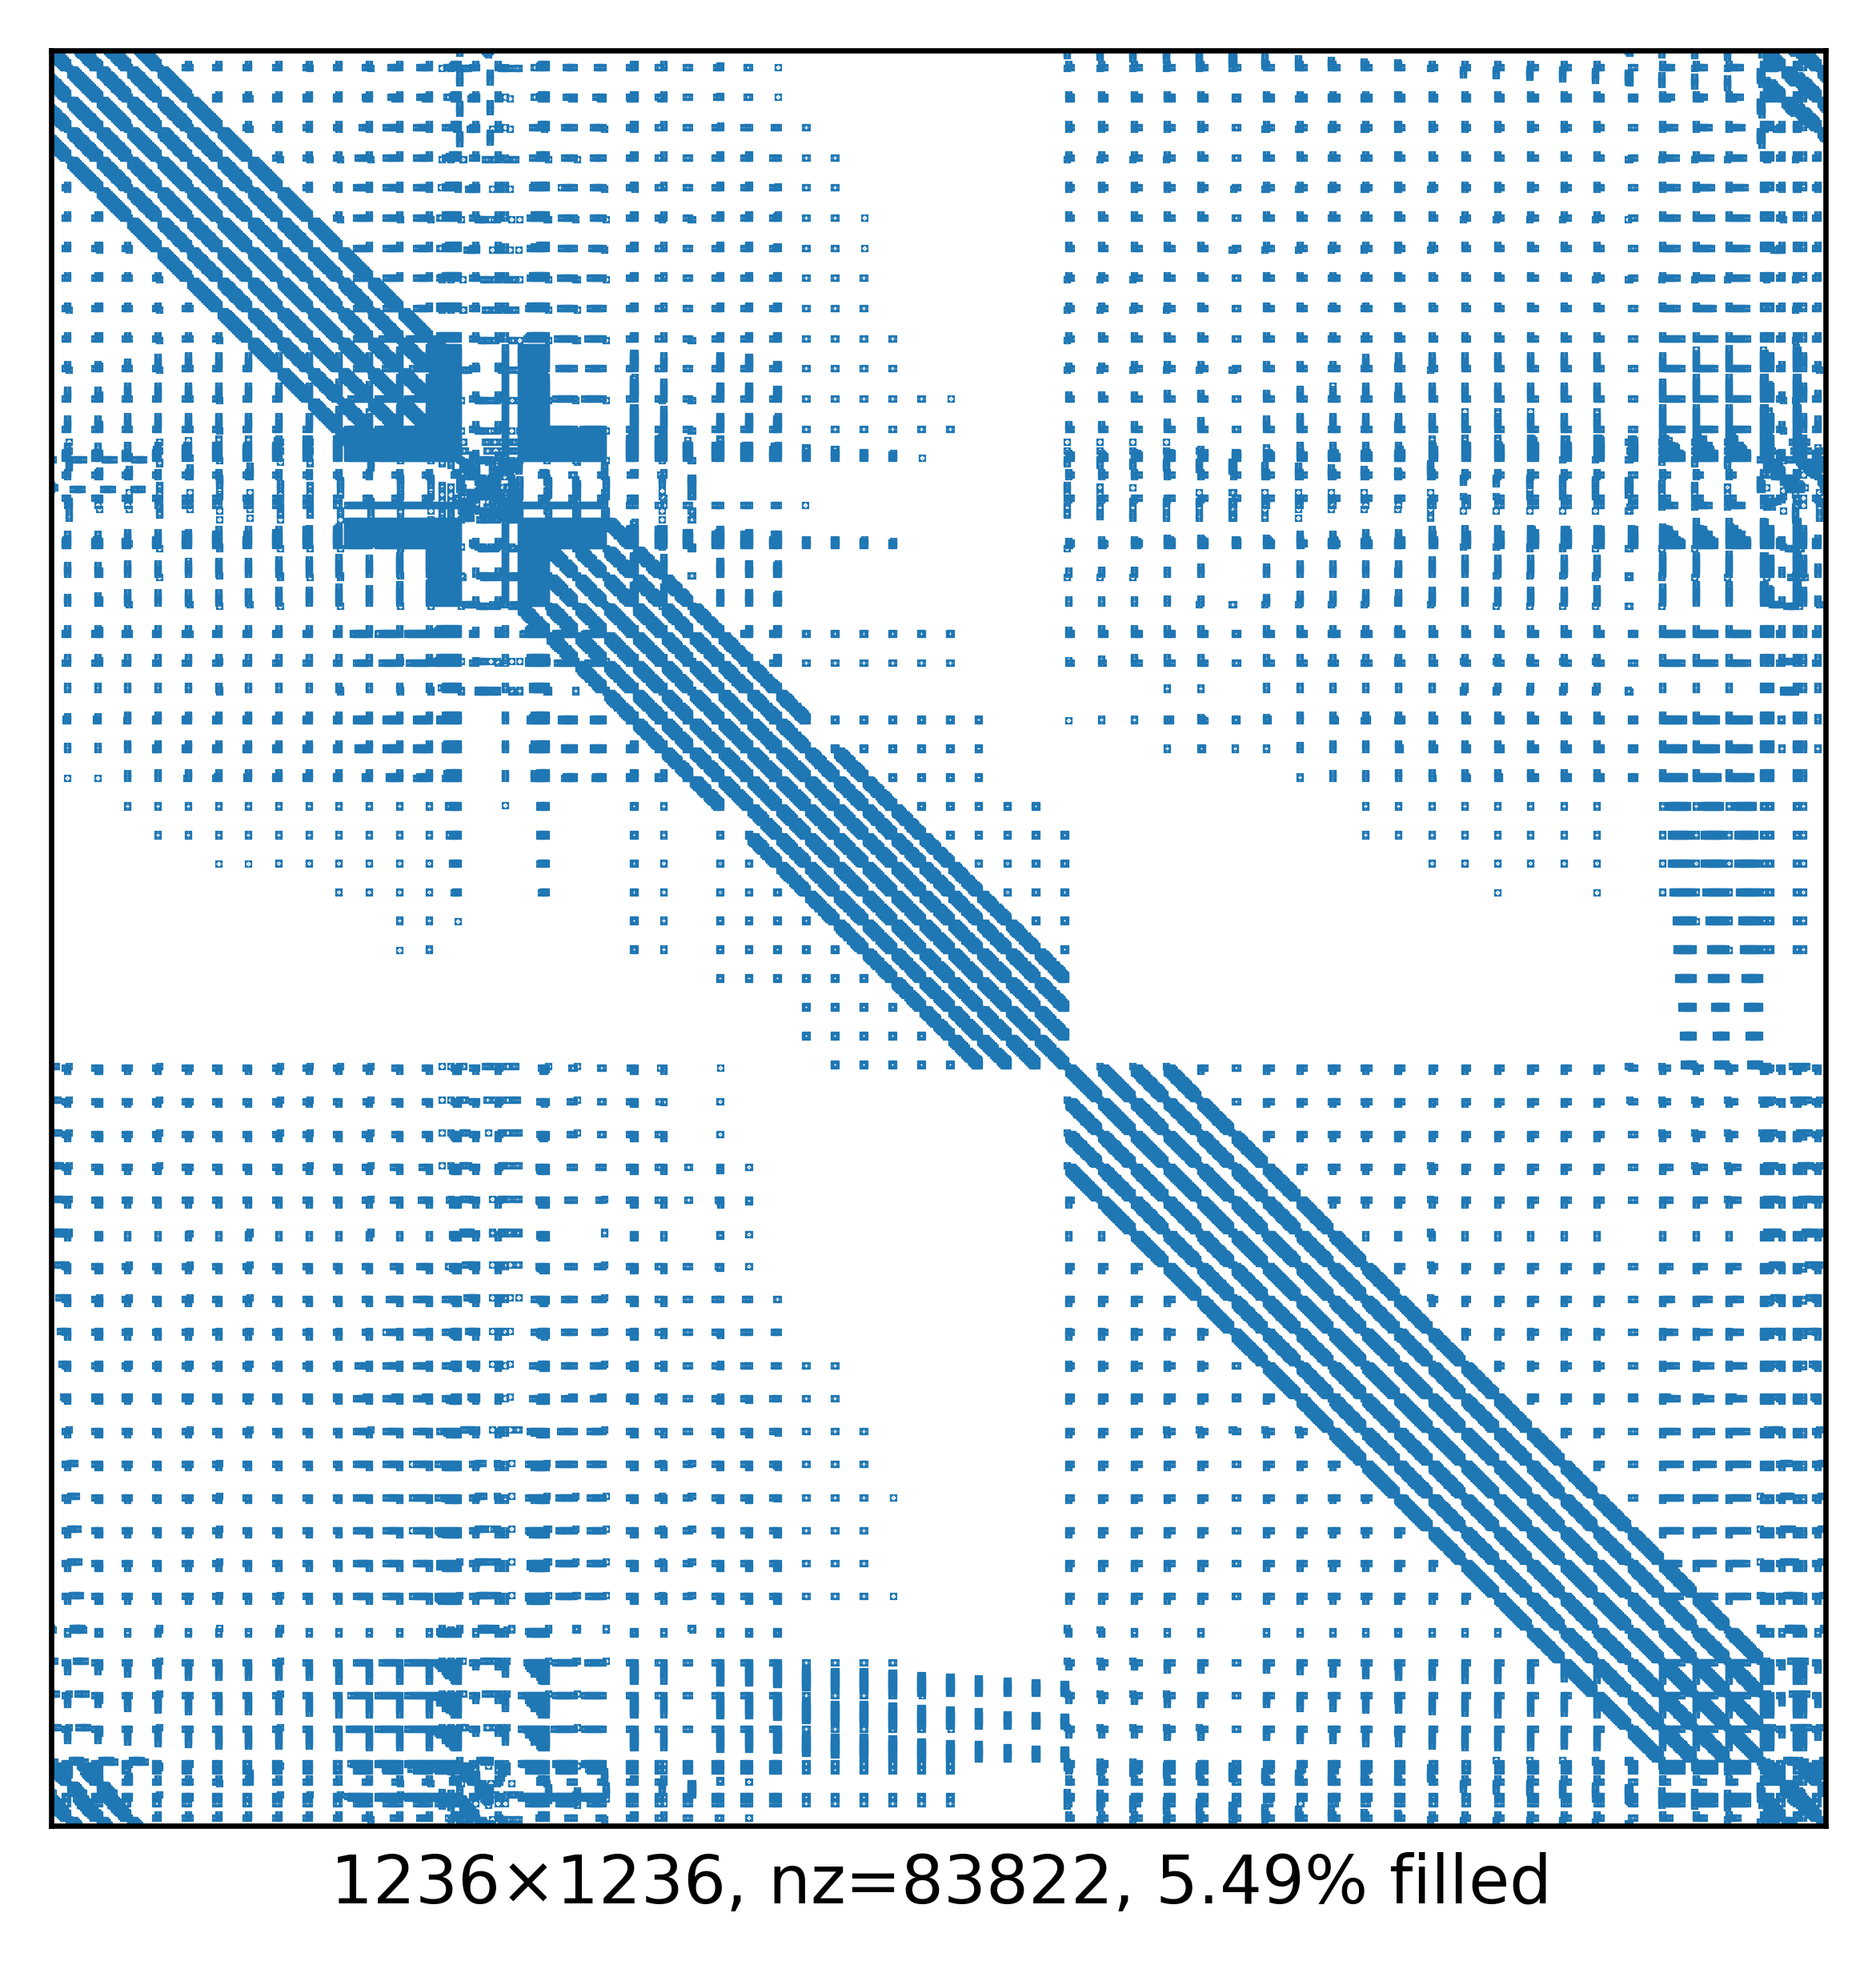
\includegraphics[width=.3\textwidth]{direct_filtered.png}} &
        \raisebox{-0.5\height}{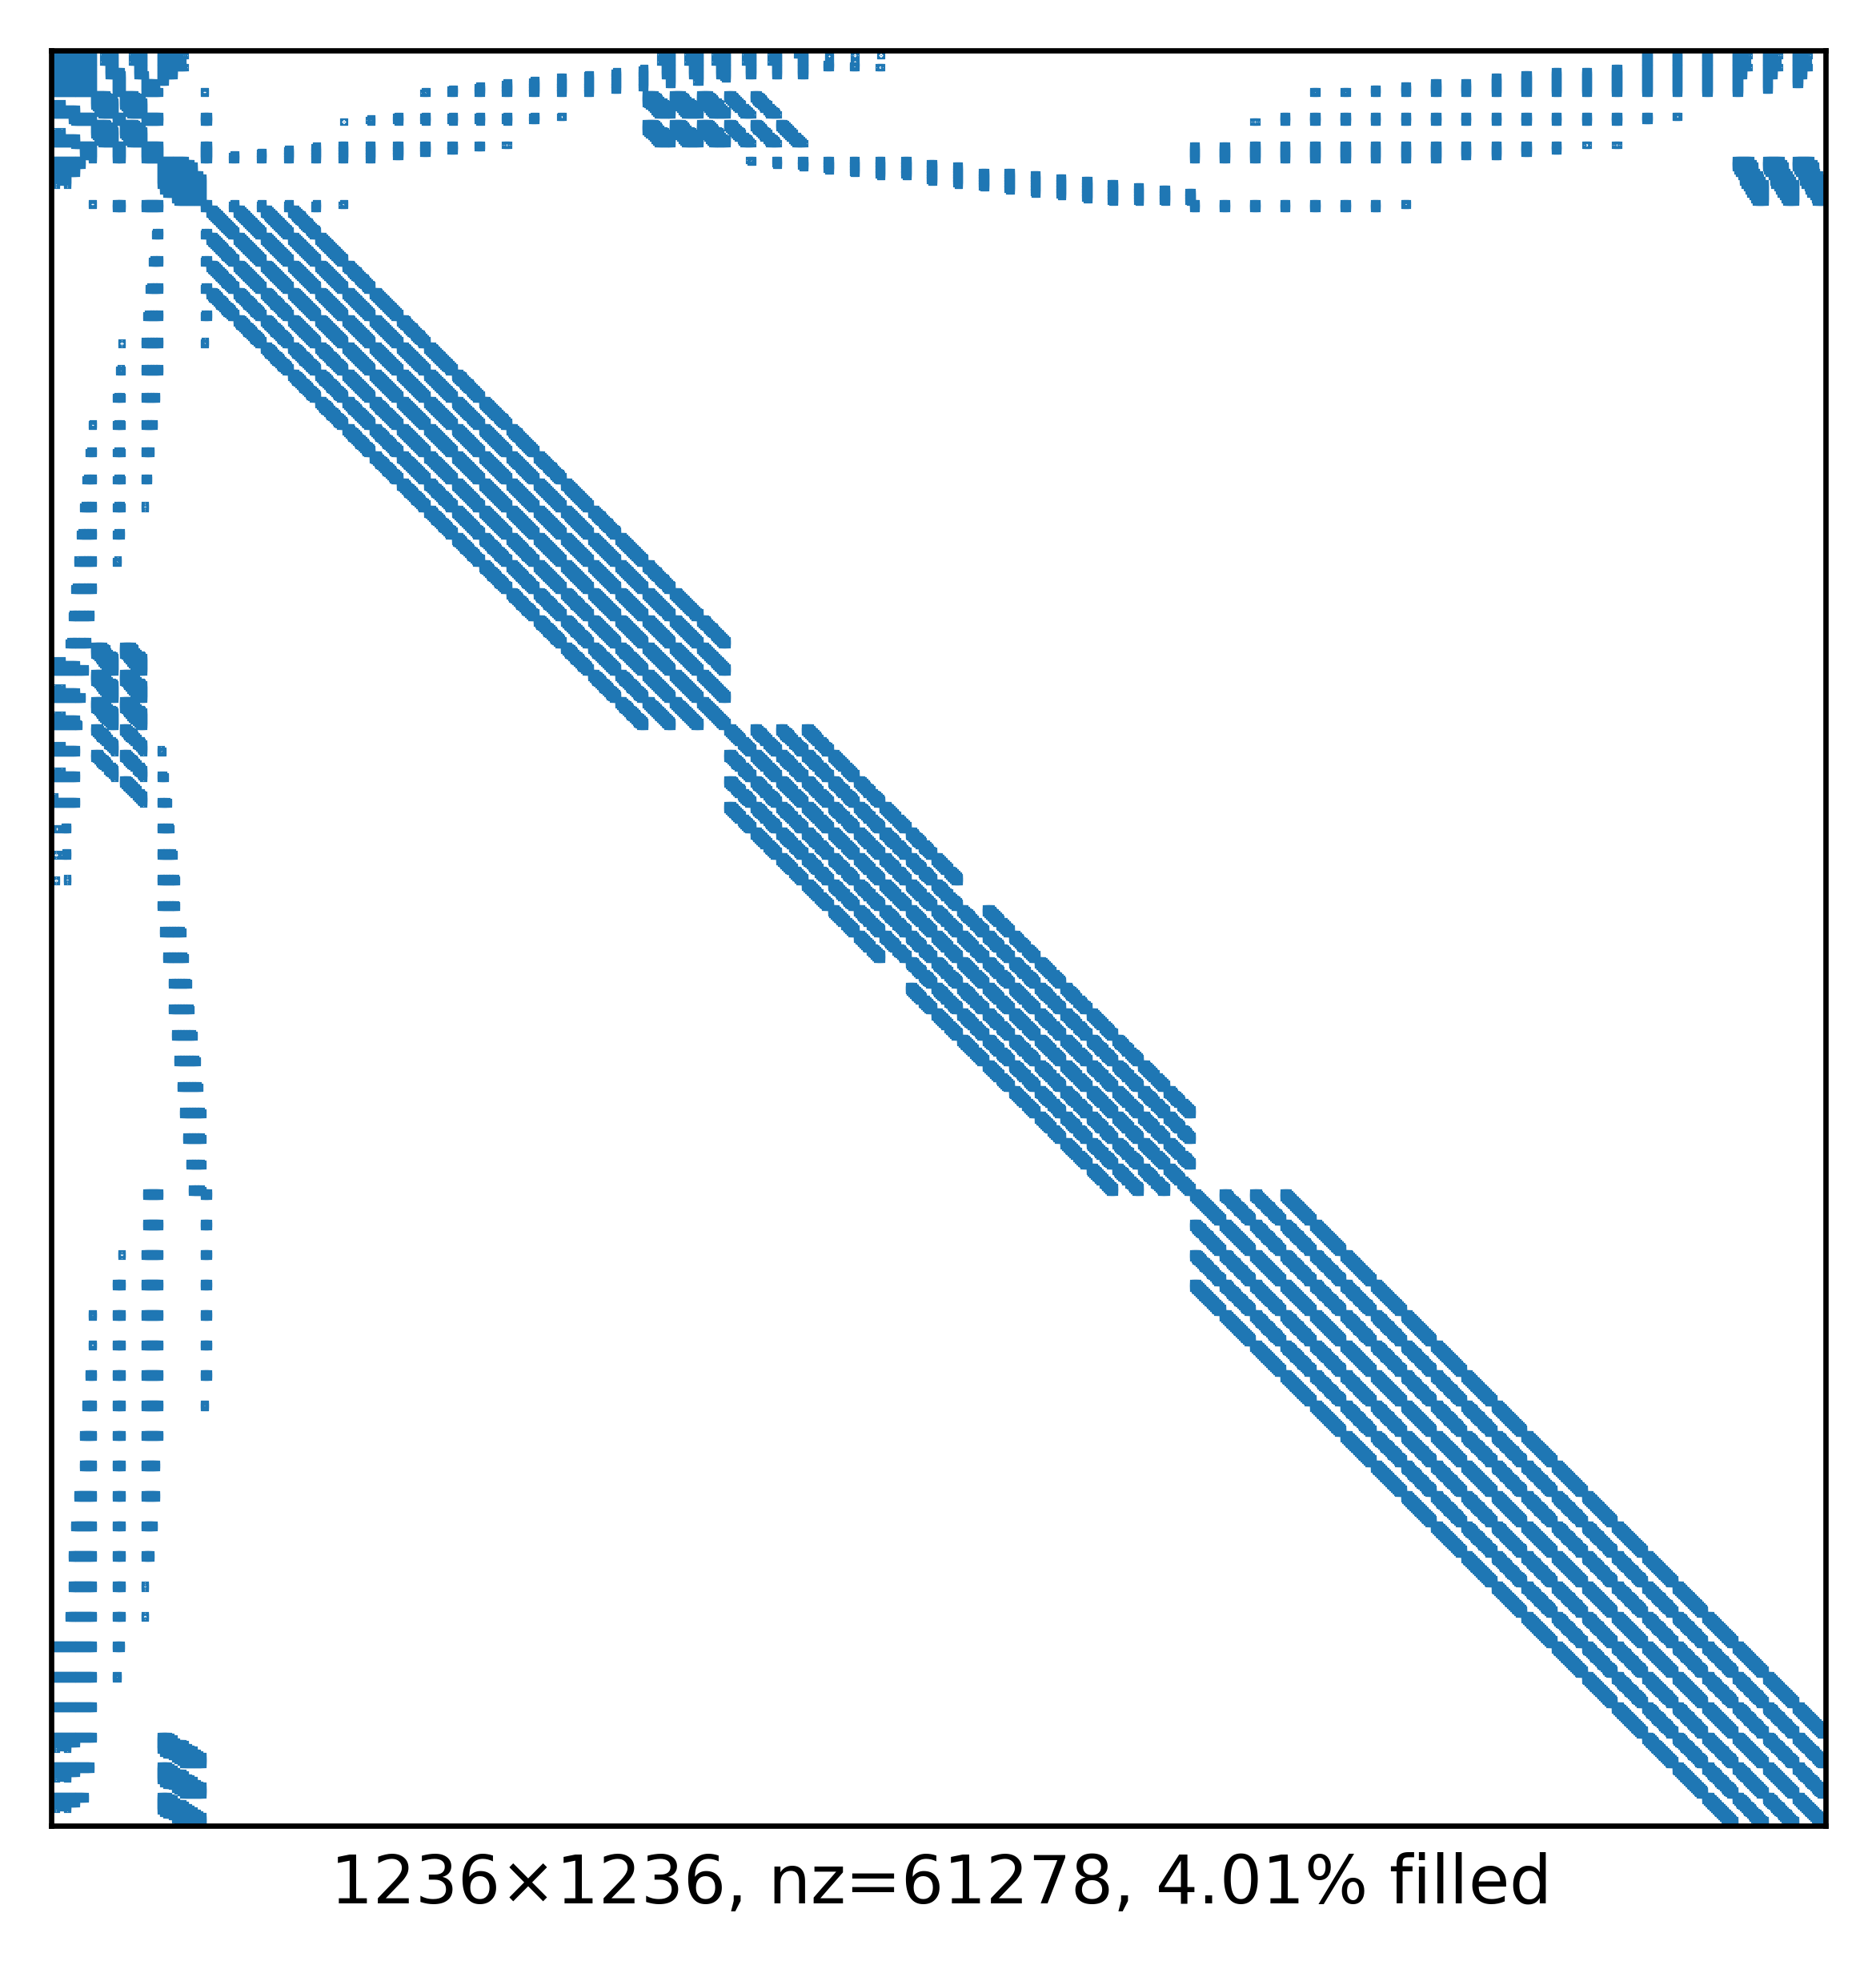
\includegraphics[width=.3\textwidth]{proposed.png}}\\
        & \scriptsize\centering Standard $\&$ Global factorization & \scriptsize\centering \Bezier dual $\&$ Global factorization & \scriptsize\centering \Bezier dual $\&$ Local factorization \\
    \end{tabular}
    \caption{Sparsity patterns of constrained stiffness matrices. Left: standard Lagrange multipliers with global factorization. Middle: \Bezier dual basis with global factorization. Right: \Bezier dual basis with localized factorization. Top: original matrix. Bottom: small absolute values ($\leq{}10^{-14}$) be pruned. All stiffness matrices are formulated for the three-patch coupling in Figure.~\ref{fig:three_planar_patches} with $3^{rd}$ order B-spline basis functions after 4 refiments. The number of non-zero entries is given by nz.}\label{fig:sparity_pattern}
\end{figure}


\section{Schedule}
\begin{table}[hbt]
    \caption{A schedule of tasks and stages of my research towards the final dissertation.}
    \hspace*{-1.5in}
	\centering
    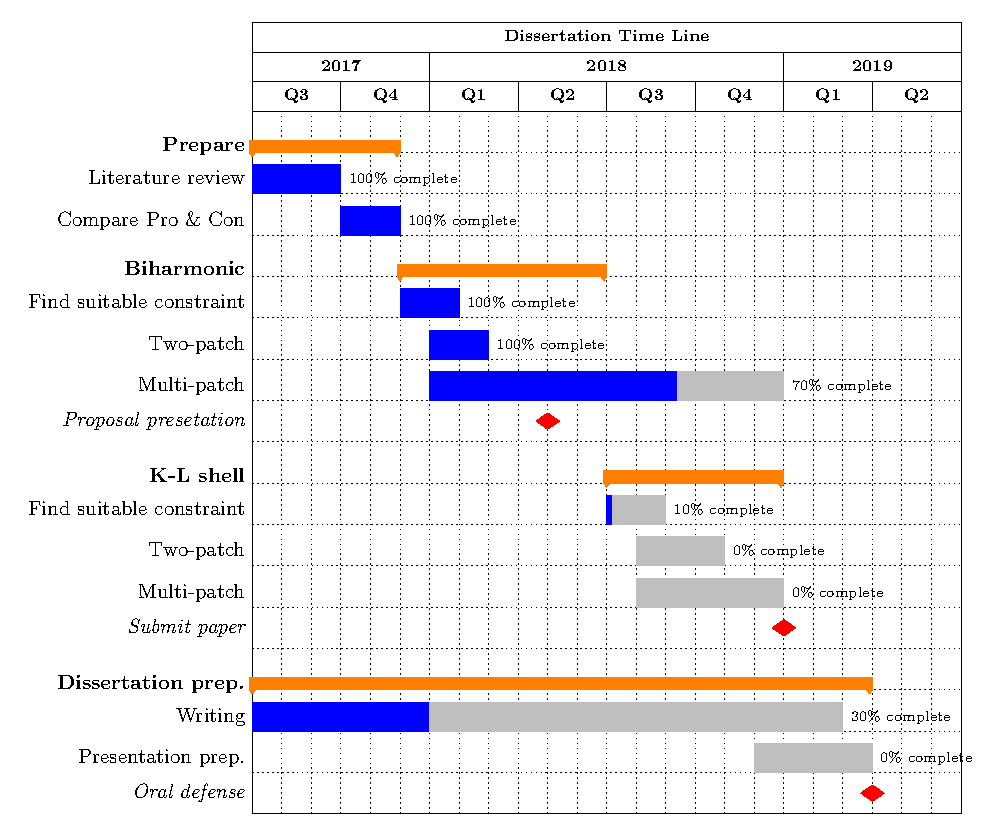
\includegraphics[width=1.5\linewidth]{schedule}\label{tab:schedule_gantt}
\end{table}
Although there are various aspects in weak $C^1/G^1$ coupling deserve a thorough study, our main focus in this stage is to extend our finding in an abstract problem (biharmonic problem) to practical problems (e.g. Kirchhoff-Love shell). Compared to the planar biharmonic problem, Kirchhoff-Love shell is a more challenging problem, as the computational domain is in $\mathbb{R}^3$ and the constraint is not isotropically applied in each direction. Hence, a more generalized constraint is needed to compromise geometries with kinks. And validations are needed for two-patch and multi-patch Kirchhoff-Love shells. Meanwhile, although we have implemented two algorithms to solve multi-patch biharmonic problems, the boundary modification method does not delivers ideal results while an additional factorization is needed for explicitly solving the null space. We will still make efforts in finding a feasible boundary modification for multi-patch coupling. A detailed time line is shown in Table.~\ref{tab:schedule_gantt}.

\clearpage
\bibliography{Zotero.bib}
\bibliographystyle{plain}


\end{document}

%%
%% End of file `elsarticle-template-1-num.tex'.